\chapter{Related Work} \label{chap:relatedwork}

\minitoc

Multi-granularity locking is a well-known solution to the problem of hierarchical locking in database systems. 
With MGL, locking a vertex in a hierarchy in a specific mode implicitly locks some or all its descendants in the same mode. 
This is a powerful concept that allows for efficient locking of hierarchical data structures without the need to explicitly lock large portions of the hierarchy.
While powerful, implementing an MGL protocol that successfully achieves this goal is non-trivial. 
% The primary challenge is an efficient computation of the ancestor-descendant relationships in the hierarchy. 
% Along with this, there are other requirements that contribute to the performance trade-offs of the locking protocol. 


% Generally, any locking approach has certain requirements and balances trade-offs between performance and correctness.
% Hierarchical locking approaches utilize several clever tricks to identify lock granularities, place locks on the vertices of the hierarchy and to ensure that the locking protocol is safe, fair and does not lead to starvation. 

The different locking approaches discussed in this chapter use different mechanisms to address the requirements specified in Section \ref{sec:requirements}, each with its own trade-offs. 
It would be appropriate to claim that no approach is all encompassing and the choice of the locking approach depends on the specific requirements of the application and the hierarchy being used. 

In this chapter, we explore some existing locking protocols and how successful they are in addressing the requirements of MGL. We present their strengths, weaknesses and the niche they occupy. Finally, we present the trade-offs between them and finally, motivate the need for a new hierarchical locking protocol which addresses the limitations of the existing protocols by classifying them into categories based on the requirements they fulfil.



\section{Existing Lock techniques}
\subsection{Level-based locks}
Level-based locking is a synchronization technique employed in hierarchical data structures to control concurrent access by just utilizing their structure. Level-based locks form lock grains based on some topological property of the hierarchy.
% Level-based locks are the simplest form of locking for uses where the hierarchy is known a priori and the semantic classification of the vertices is fixed. 
% Fixed-grain locking associates a fixed guard with a set of target vertices in the hierarchy which from the grain of that guard.
% The two extremes of locking discussed in Chapter \ref{chap:background} are variants of fixed-grain locking. 
One approach to level-based locking is to associate a lock guard per level of the hierarchy. This level is determined by the depth of vertices in the hierarchy. Vertices with the same depth are associated with a single lock guard.
As shown in Figure \ref{fig:level_locks}, the hierarchy is divided into levels based on the depth of the vertices and a lock guard is associated with each level. 
This guard protects all vertices in that level.
To lock a target vertex, a thread acquires the lock associated with the level of that target and locks all the vertices in that level.
For example, in Figure \ref{fig:level_locks}, in order to lock target vertex $D$, vertices $E$, $F$ and $G$ are implicitly locked as well since they are in the same level and protected by the same guard as $D$.

\begin{figure}[h]
    \centering
    \captionsetup{justification=centering}
    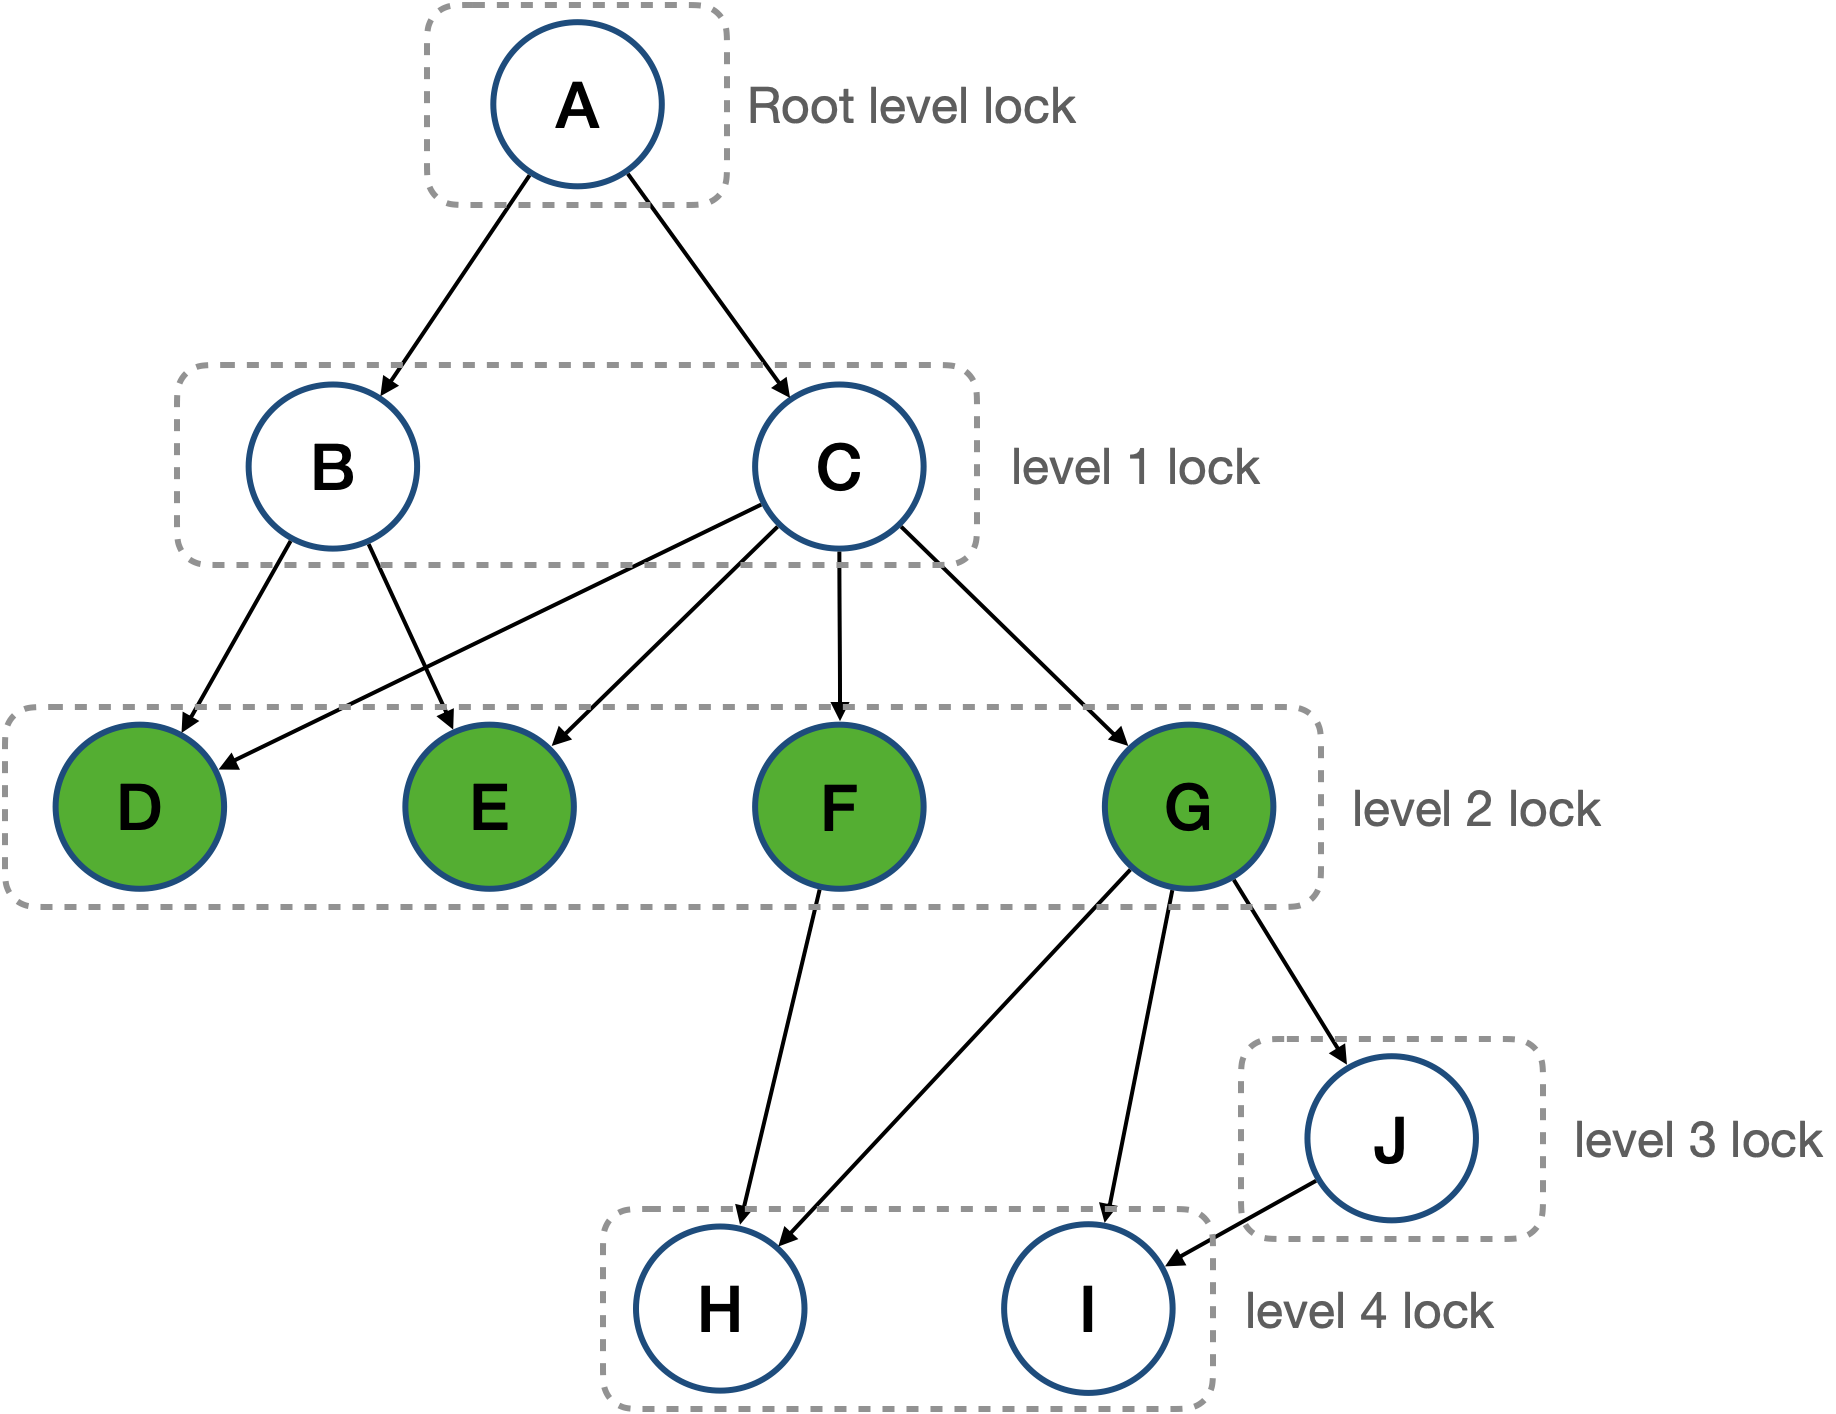
\includegraphics[width=0.7\textwidth]{figures/FixedGrainLevelLocks.png}
    \caption{Hierarchical locks with fixed grains per level and a lock on level 2}
    \label{fig:level_locks}
\end{figure}

Level-based locks fulfil only requirement \textbf{R1} since the lock guard is fixed for a set of vertices. 
However, since the lock grain is fixed by level, acquiring a lock on a specific level implicitly locks all the vertices in that level. This leads to unnecessary conflicts between conflicts that access disjoint sets of vertices in the same level. 
For example, consider two threads $T_1$ and $T_2$ that want to lock vertices $D$ and $E$ respectively.
Since the lock guard for level 2 is the same, $T_1$ and $T_2$ will always conflict with each other even though they are accessing different vertices. 

% The lock guard for a request is not guaranteed to be optimal when using fixed-grain locks. 
% Depending on the lock grains chosen, the ancestor-descendant relationship may not be correctly identified. 
% This leads to unnecessary conflicts and can lead to performance degradation.
% For example, $D$ and $E$ are not related by an ancestor-descendant relationship and hence, under an effective MGL protocol, should not conflict.


\subsection{Intention Lock}

Intention locks are used to coordinate concurrent access by indicating a thread’s intention to acquire more fine-grain locks within a hierarchy. Unlike traditional locks that are placed directly on lock targets, intention locks are acquired at higher levels of a hierarchy to signal that a thread plans to acquire finer-grained locks on specific target vertices which exist deeper in the hierarchy. These intention locks protect the paths that lead to the target vertices from the root. By guarding these paths, intention locks ensure that the target vertices can be accesses exclusively by writers.

Intention locking was one of the first approaches to hierarchical locking designed to efficiently meet requirements \textbf{R1} and \textbf{R3}. \citet{gray1975granularity} introduced three new lock modes: IS (Intention Shared), IX (Intention Exclusive), and SIX (Shared Intention Exclusive), which allow a thread to signify its intention to acquire a shared or exclusive lock on a descendant of a vertex locked under IS, IX, or SIX modes, respectively. In the intention lock protocol, a thread acquires these intention locks on all the paths from the root to the lock target, which is then locked in either a shared (S) or exclusive (X) mode. Thus, all the ancestors of a target vertex are locked in an intention mode, and the target vertex is locked in a shared or exclusive mode.

The protocol requires that threads place these locks in a depth-first manner. This ordering ensures that two concurrent threads trying to lock the same target will always acquire the locks in the same order, allowing them to detect conflicts deterministically. Table \ref{tab:intention_locks} shows the compatibility matrix for the intention locks.


% Intention locking is one of the first approaches to hierarchical locking that attempts to address the requirements \textbf{R1} and \textbf{R3} with efficiency.
% \citet{gray1975granularity} introduce three new lock modes: IS (Intention Shared), IX (Intention Exclusive) and SIX (Shared Intention Exclusive) which signify the intention of a thread to acquire a shared or exclusive lock on a descendant of a vertex locked under IS, IX or SIX modes respectively.
% Intention lock protocol works by acquiring the aforementioned intention locks on the paths from the root to the lock target. The lock target is then locked in a shared (S) or exclusive (X) mode. These locks are always placed in a top-down, depth first manner. Owing to this, two concurrent threads, trying to lock the same lock target will always acquire the locks in the same order and detect a conflict. Table \ref{tab:intention_locks} shows the compatibility matrix for the intention locks.


\begin{table}[h]
    \centering
    \captionsetup{justification=centering}
    \begin{tabular}{c|ccccccc}
        \textbf{Mode} & \textbf{NL} & \textbf{IS} & \textbf{IX} & \textbf{S} & \textbf{SIX} & \textbf{X}\\
        \hline
        \textbf{NL} & \cellcolor{green!25} Y & \cellcolor{green!25} Y & \cellcolor{green!25} Y & \cellcolor{green!25} Y & \cellcolor{green!25} Y & \cellcolor{green!25} Y \\
        \textbf{IS} &  \cellcolor{green!25} Y & \cellcolor{green!25} Y & \cellcolor{green!25} Y & \cellcolor{green!25} Y & \cellcolor{green!25} Y & \cellcolor{red!25} N \\
        \textbf{IX} &  \cellcolor{green!25} Y & \cellcolor{green!25} Y & \cellcolor{green!25} Y & \cellcolor{red!25} N & \cellcolor{red!25} N & \cellcolor{red!25} N \\
        \textbf{S} &  \cellcolor{green!25} Y & \cellcolor{green!25} Y & \cellcolor{red!25} N & \cellcolor{green!25} Y & \cellcolor{red!25} N & \cellcolor{red!25} N \\
        \textbf{SIX} &  \cellcolor{green!25} Y & \cellcolor{green!25} Y & \cellcolor{red!25} N & \cellcolor{red!25} N & \cellcolor{red!25} N & \cellcolor{red!25} N \\
        \textbf{X} &  \cellcolor{green!25} Y & \cellcolor{red!25} N & \cellcolor{red!25} N & \cellcolor{red!25} N & \cellcolor{red!25} N & \cellcolor{red!25} N \\
    \end{tabular}
    \caption{Compatibility matrix for intention lock modes. \textbf{NL}: NoLock, \textbf{IS}: Intention Shared, \textbf{IX}: Intention Exclusive, \textbf{S}: Shared, \textbf{SIX}: Shared Intention Exclusive, \textbf{X}: Exclusive}
    \label{tab:intention_locks}
\end{table}



\begin{figure}[h]
    \centering
    \captionsetup{justification=centering}
    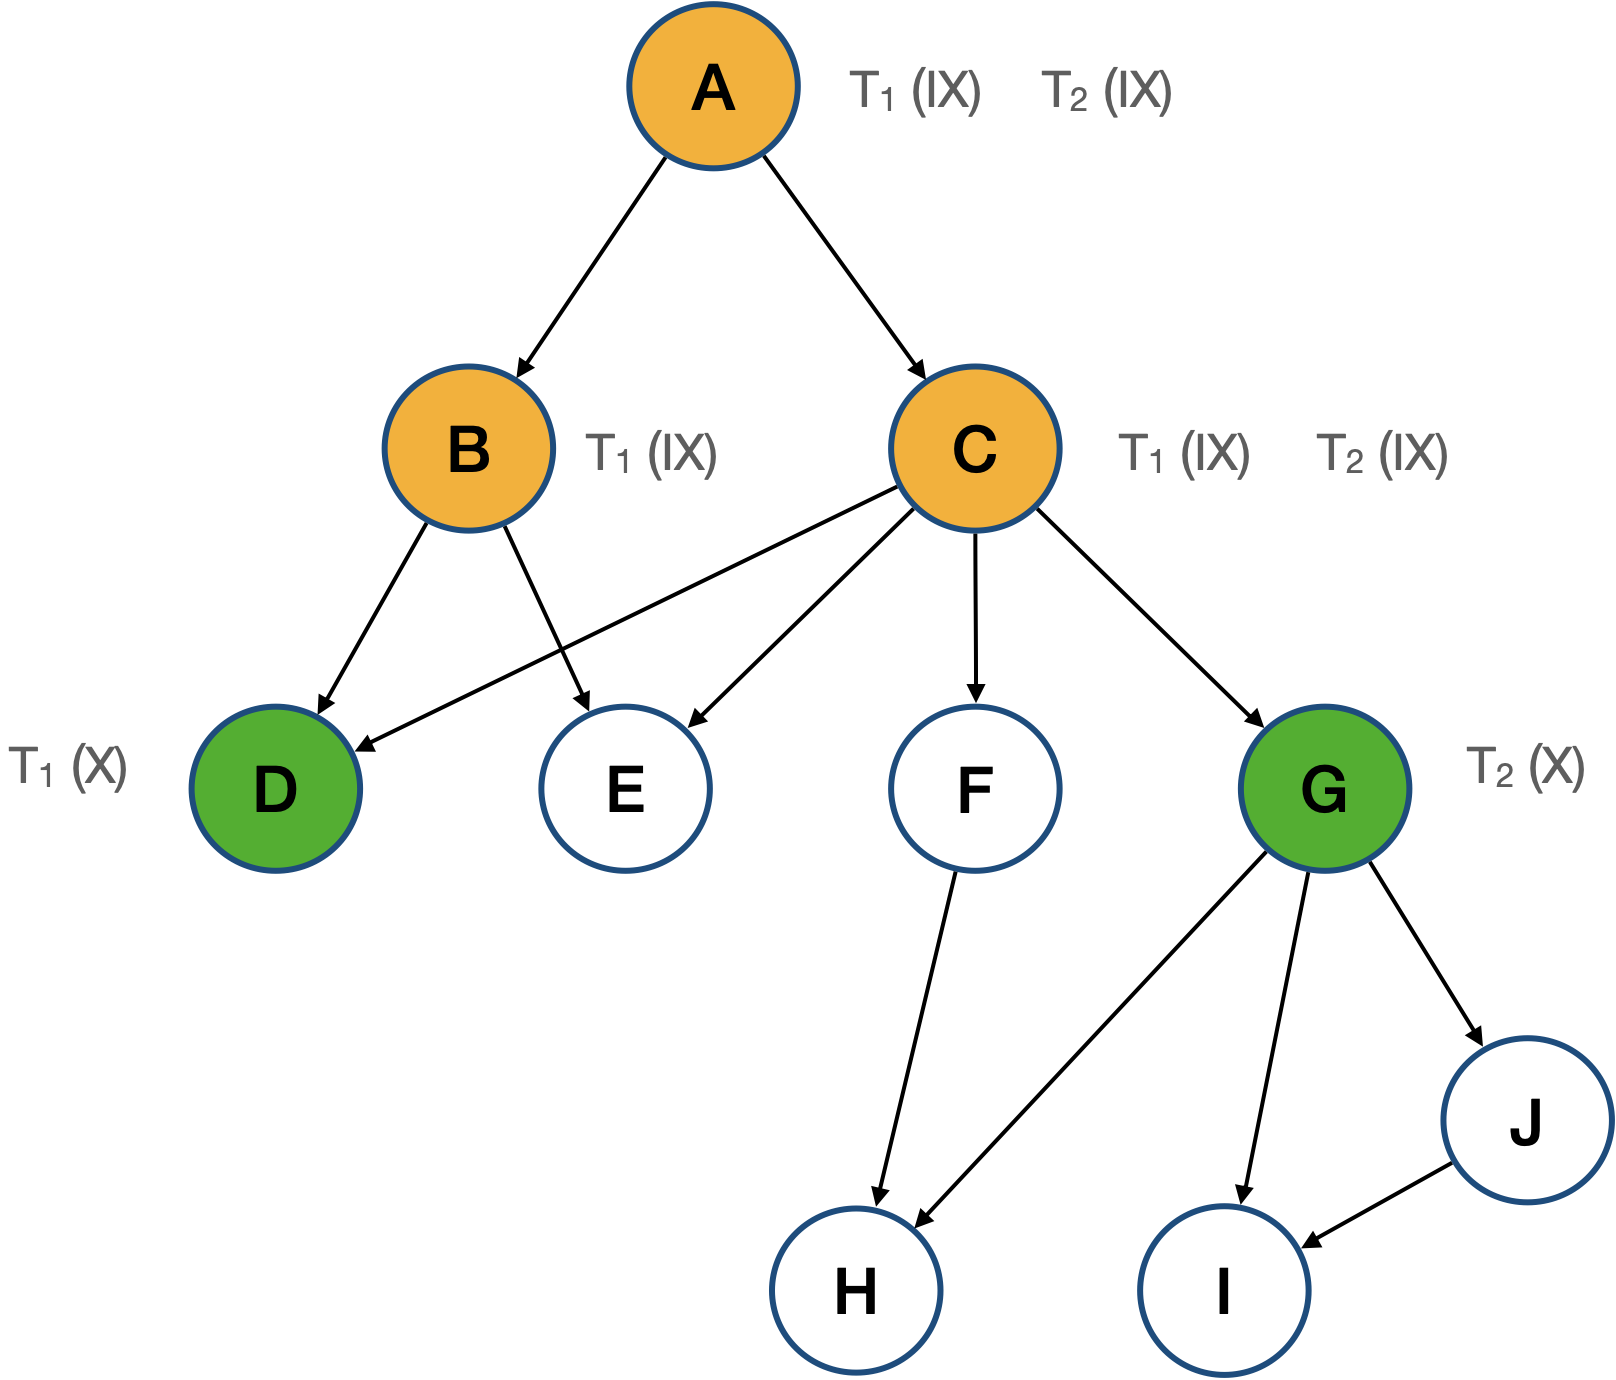
\includegraphics[width=0.6\textwidth]{figures/IntentionLockExample.png}
    \caption{Multi granularity locking via Intention locks. \\ $T_1$ takes an exclusive lock on vertex $D$ and $T_2$ takes an exclusive lock on vertex $G$ }
    \label{fig:intention_lock_example}
\end{figure}

Consider the example in Figure \ref{fig:intention_lock_example} where a thread $T_1$ wishes to acquire an exclusive lock (X) on target vertex $D$ and another thread, $T_2$ on target vertex $G$. 
% Since $D$ and $G$ are not related by an ancestor-descendant relationship, they should not conflict.
With intention locks, both threads start from the root i.e. $A$ and acquire intention exclusive locks (IX) on the vertices from the root to their lock targets i.e. $D$ and $G$ respectively. 
Let's assume that $T_1$ is faster than $T_2$ and manages to acquire its locks first. 
$T_1$ acquires $IX$ on vertices $A$, $B$ and $C$, in this order, and acquires an exclusive lock on $D$. 

When $T_2$ tries to acquire a lock on $G$, it acquires IX on vertices $A$ and $C$, in this order, before trying to acquire a lock on $G$. 
When $T_2$ tries to acquire a lock on $A$, it encounters a pre-existing  IX lock acquired by $T_1$. 
Since two IX locks are compatible, as seen in Table \ref{tab:intention_locks}, $T_2$ can acquire the IX lock on $A$.
Similarly, $T_2$ can acquire the IX lock on $C$ and then proceed to acquire an exclusive lock on $G$.


By locking the vertices on the path to the target vertex under IS and IX modes, always in a depth-first manner, 
intention locking protocol correctly identifies lock grain overlaps. 
However, this process requires multiple traversals from the root to the lock target so that all paths can be locked. 
In the example of Figure \ref{fig:intention_lock_example}, $T_1$ must perform the following two traversals:

\begin{itemize}
    \item $A \rightarrow B \rightarrow D$
    \item $A \rightarrow C \rightarrow D$
\end{itemize}

In a tree, every vertex is reachable from the root via a unique path. 
This, however, is not the case with DAGs.
In DAGs, as the number of paths from the root to a target vertex increases, the number of traversals required to acquire an S or X lock on that vertex also increases because intention locks are to be acquired on all paths to the target vertex.
This leads to a significant performance degradation. Along with the added performance penalty, the order in which multiple paths are traversed needs to be deterministic to prevent deadlocks.  

So, while intention locks fulfil requirements \textbf{R1} and \textbf{R2}, requirement \textbf{R3} incurs a significant performance penalty. 

\subsection{DomLock}
DomLock \cite{kalikar2016domlock} is a MGL technique that uses the concept of dominators to identify lock grains instead of relying on explicitly locking paths that lead to a target. A dominator is a vertex that lies on all the paths from the root to a target vertex $v$ and is thus an effective lock guard for its descendants since locking a dominator is sufficient to lock all the paths to $v$ and the descendants of $v$. 

\begin{definition}[Dominator]
    A vertex $d$ is a dominator of another vertex $v$ if all the paths from root to $v$ pass through d.
\end{definition}

A vertex can have several dominators in a hierarchy. 
In order to maximize concurrency, by minimizing the number of locks required for correct exclusive access, DomLock uses the dominator of maximum depth as the lock guard. This dominator is called the immediate dominator. 


% Dominator based locking (DomLock)  uses dominators to identify the ancestor descendant relationship in a hierarchy. DomLock finds a partial ordering of vertices in the hierarchy based on the ancestor-descendant relationship between them. To this end, DomLock uses the concept of dominators and immediate dominators. 


\begin{definition}[Immediate Dominator]
    Immediate Dominator: A dominator $d$ is an immediate dominator of another vertex $v$ if there exists no other dominator for $v$ on the paths between $d$ and $v$.
\end{definition}

This immediate dominator is the deepest vertex that lies on all paths from the root of the hierarchy to a target vertex. Therefore, it is sufficient to lock this immediate dominator to lock all the paths to the target vertex and its descendants since, any traversal to the target vertex or its descendants shall encounter the immediate dominator.

\paragraph{Labelling through numeric intervals}
In order to identify the dominators of a vertex more efficiently, DomLock uses a labelling scheme that assigns a pair of integers to each vertex. This pair, called the \emph{interval} of the vertex is denoted  $I_v = [l_v, r_v]$. 
This interval $I_v$ subsumes ($\prec$) the intervals of all the descendants of $v$. Subsumption is defined as follows:
\begin{equation}
    u \text{ is a dominator of } v \iff I_u \prec I_v \iff l_v \leq l_u \land r_v \geq r_u
\end{equation}

% It is such that $l_v \leq l_u$ and $r_v \geq r_u$ for all vertices $u$ that are descendants of $v$. 

These intervals are computed by performing a post-order traversal of the hierarchy. Consider the example in Figure \ref{fig:domlock_example_locked}. The leaves are labelled with unit intervals. For example, vertex $D$ is labelled with the interval $[1, 1]$ since it is the first vertex in the post-order traversal. 

\begin{figure}
    \centering
    \captionsetup{justification=centering}
    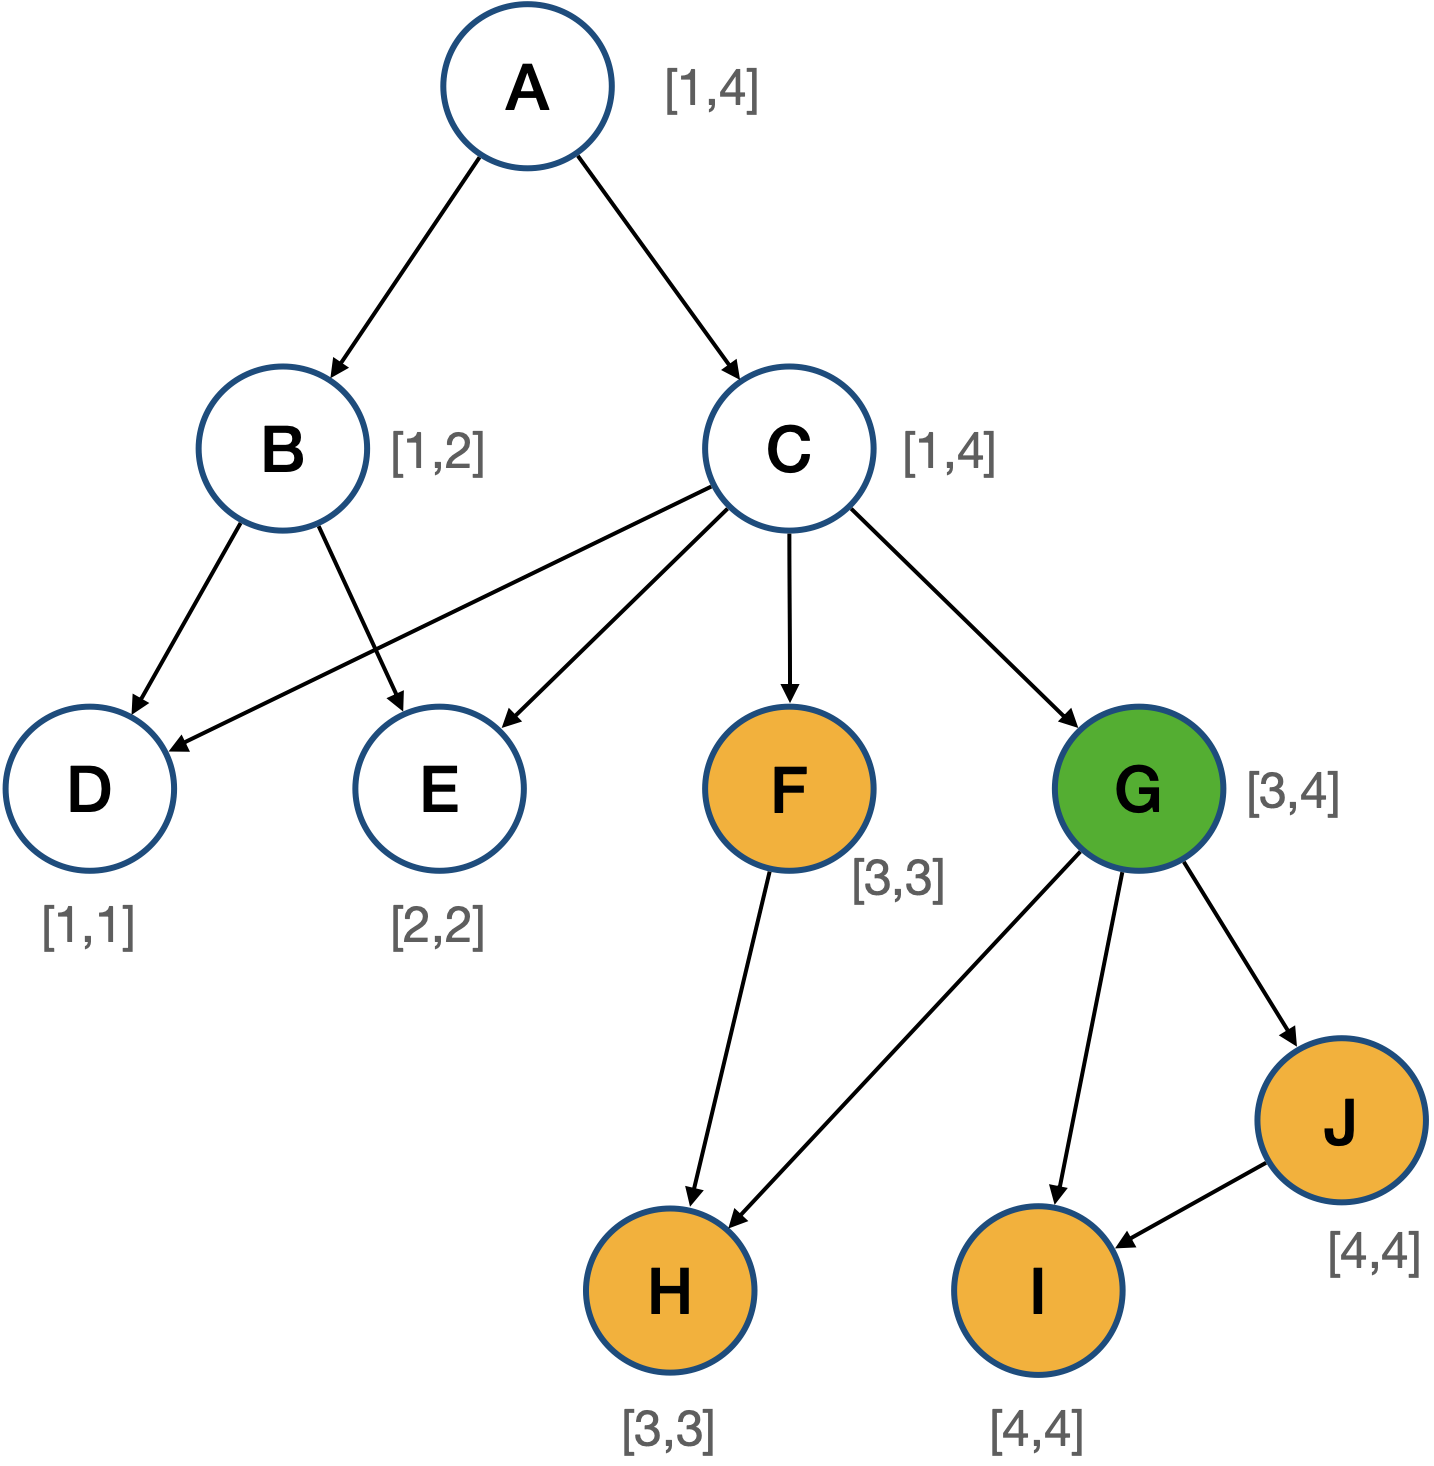
\includegraphics[width=.6\textwidth]{figures/domlock_example_with_lock.png}
    \caption{Hierarchy labelled with DomLock intervals and DomLock on $G$ (lock guard) with the grain of the grain of the lock (yellow).}
    \label{fig:domlock_example_locked}
\end{figure}
For an internal vertex, the interval is computed via its children's. The $l$ value of an internal vertex $v$ is the minimum of the $l$ values of its children and the $r$ value of an internal vertex $v$ is the maximum of the $r$ values. For example, in Figure \ref{fig:domlock_example_locked}, vertex $G$ has three children $H$, $I$ and $J$. The interval of $G$ is $[3,4]$ since the minimum $l$ value of its children is 3 and the maximum $r$ value of its children is 4.  In turn, G $\prec$ \{H, I, J\}
% \begin{figure}[h]
%     \centering
%     \captionsetup{justification=centering}
%     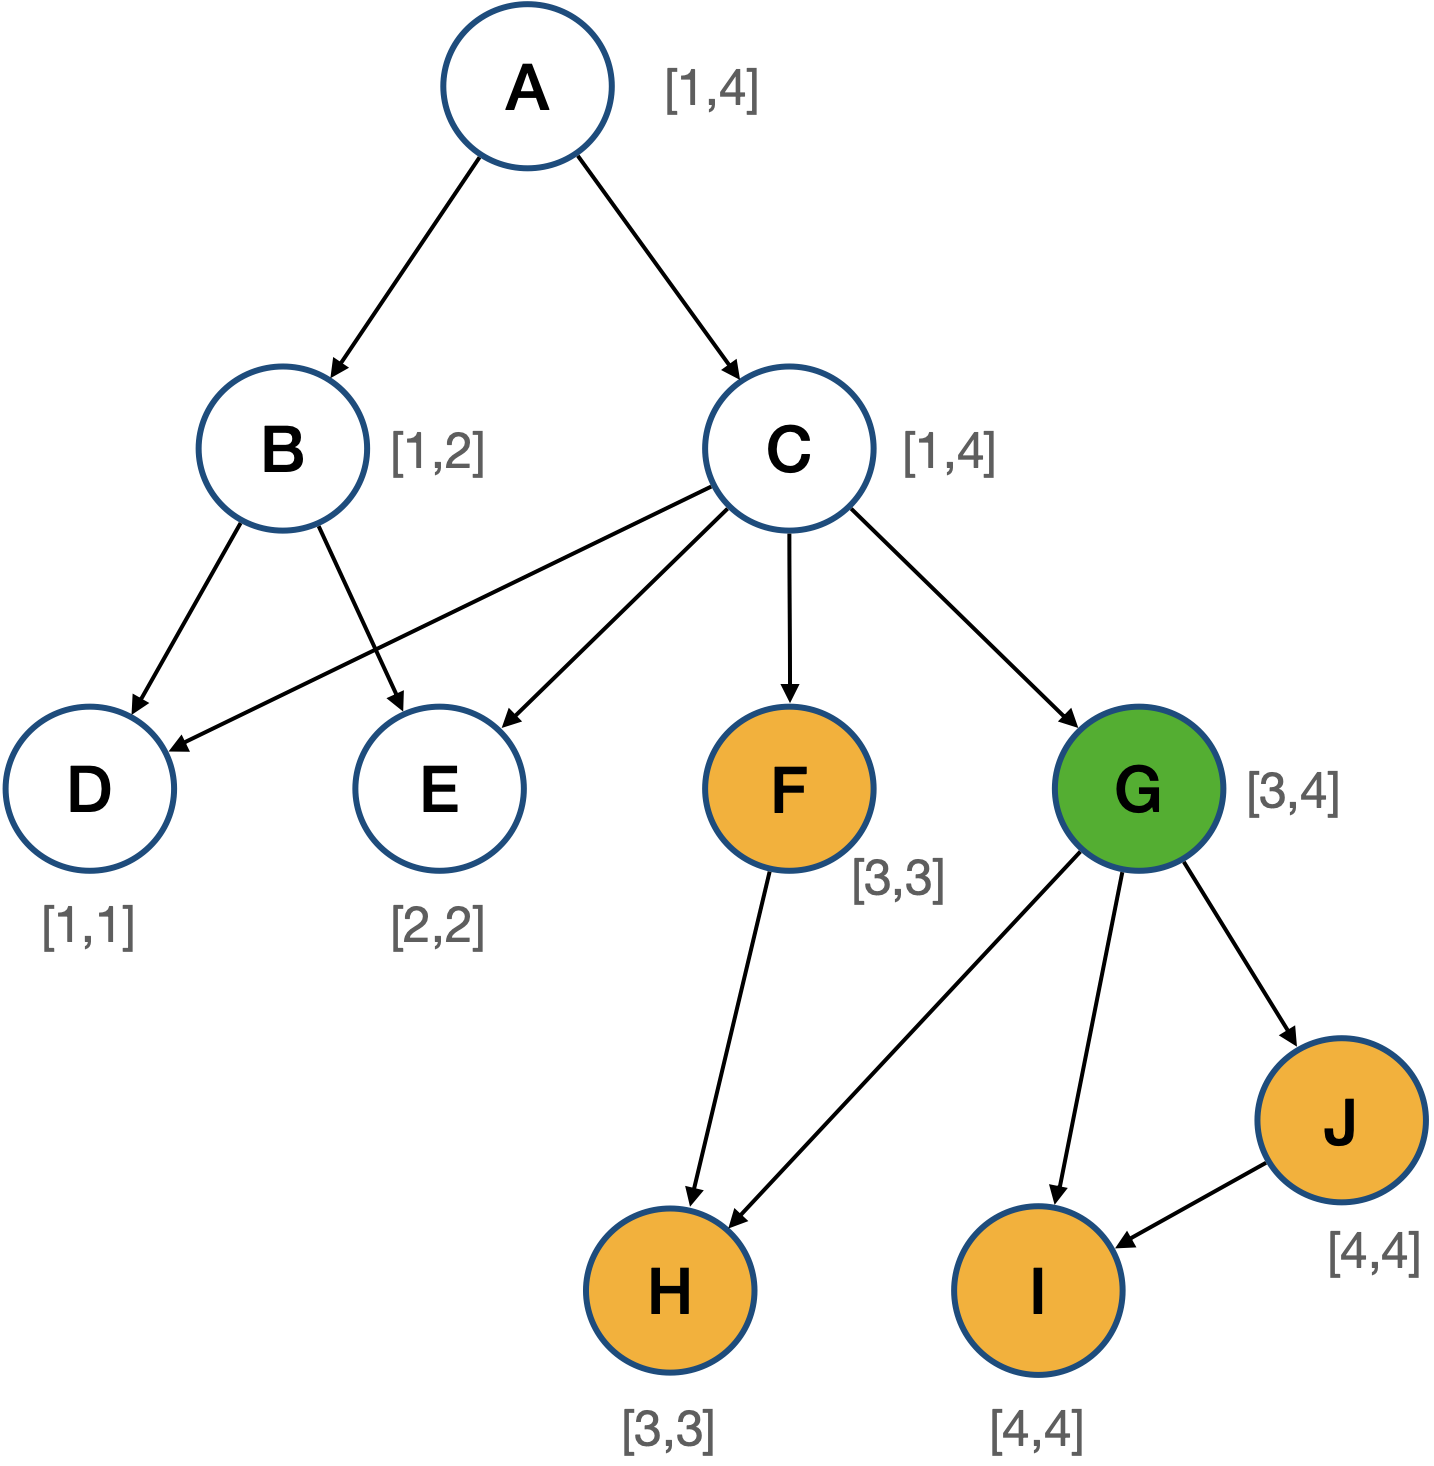
\includegraphics[width=0.5\textwidth]{figures/domlock_example_with_lock.png}
%     \caption{DomLock on guard $G$ with the grain of the grain of the lock (yellow).}
%     \label{fig:domlock_example_locked}
% \end{figure}

\paragraph{Lock Grain identification}

Lock grain identification in DomLock is based on the intervals of the vertices. The grain of a lock guard $g$ contains any vertex $v$ such that $v$ is a descendant of $g$ and $I_g \prec I_v$. 
In practice, this involves a depth first search from the root of the hierarchy to identify the deepest vertex that satisfies the subsumption property to ensure that the granularity is as small as possible by locking the immediate dominator.
% A vertex $u$ subsumes another vertex $v$ when their intervals overlap i.e. $l_v \leq r_u \land l_u \leq r_v$. The lock grain of a guard $u$ is the set of vertices that have an overlapping interval with the interval of $u$. 
For example, in Figure \ref{fig:domlock_example_locked}, the grain of $G$ contains $F$, $H$, $I$ and $J$ since the interval of $G$ overlaps with the intervals of $F$, $H$, $I$ and $J$ which are $[3,3]$, $[3,3]$, $[4,4]$ and $[4,4]$ respectively.

Herein lies the first major drawback of DomLock. 
Due to the subsumption property and the manner in which numeric intervals are assigned to vertices, \emph{False subsumptions} can occur. 
Subsumption is a property that exists between two vertices related via an ancestor-descendant relationship. 
A \emph{False subsumption} occurs when the intervals of two vertices overlap, but they are not related by an ancestor-descendant relationship. 
For example, in Figure \ref{fig:domlock_example_locked}, $G$ is the dominator of $F$ but $F$ is not a descendant of $G$. 
Sometimes, due to a false subsumption disjoint subgraphs are locked together. 
This leads to spurious lock conflicts and consequently, performance degradation. 

\paragraph{Label recomputation}
Another drawback of DomLock is that it does not support dynamic hierarchies. 
Since intervals are used to identify lock grains and determine the ancestor-descendant relationship, the intervals of the vertices have to be recomputed when a structural modification occurs.
% The intervals of the vertices are computed once via a post-order traversal. When a vertex is added or removed from the hierarchy, this computation has to be redone. 

\begin{figure}[h]
    \centering
    \captionsetup{justification=centering}
    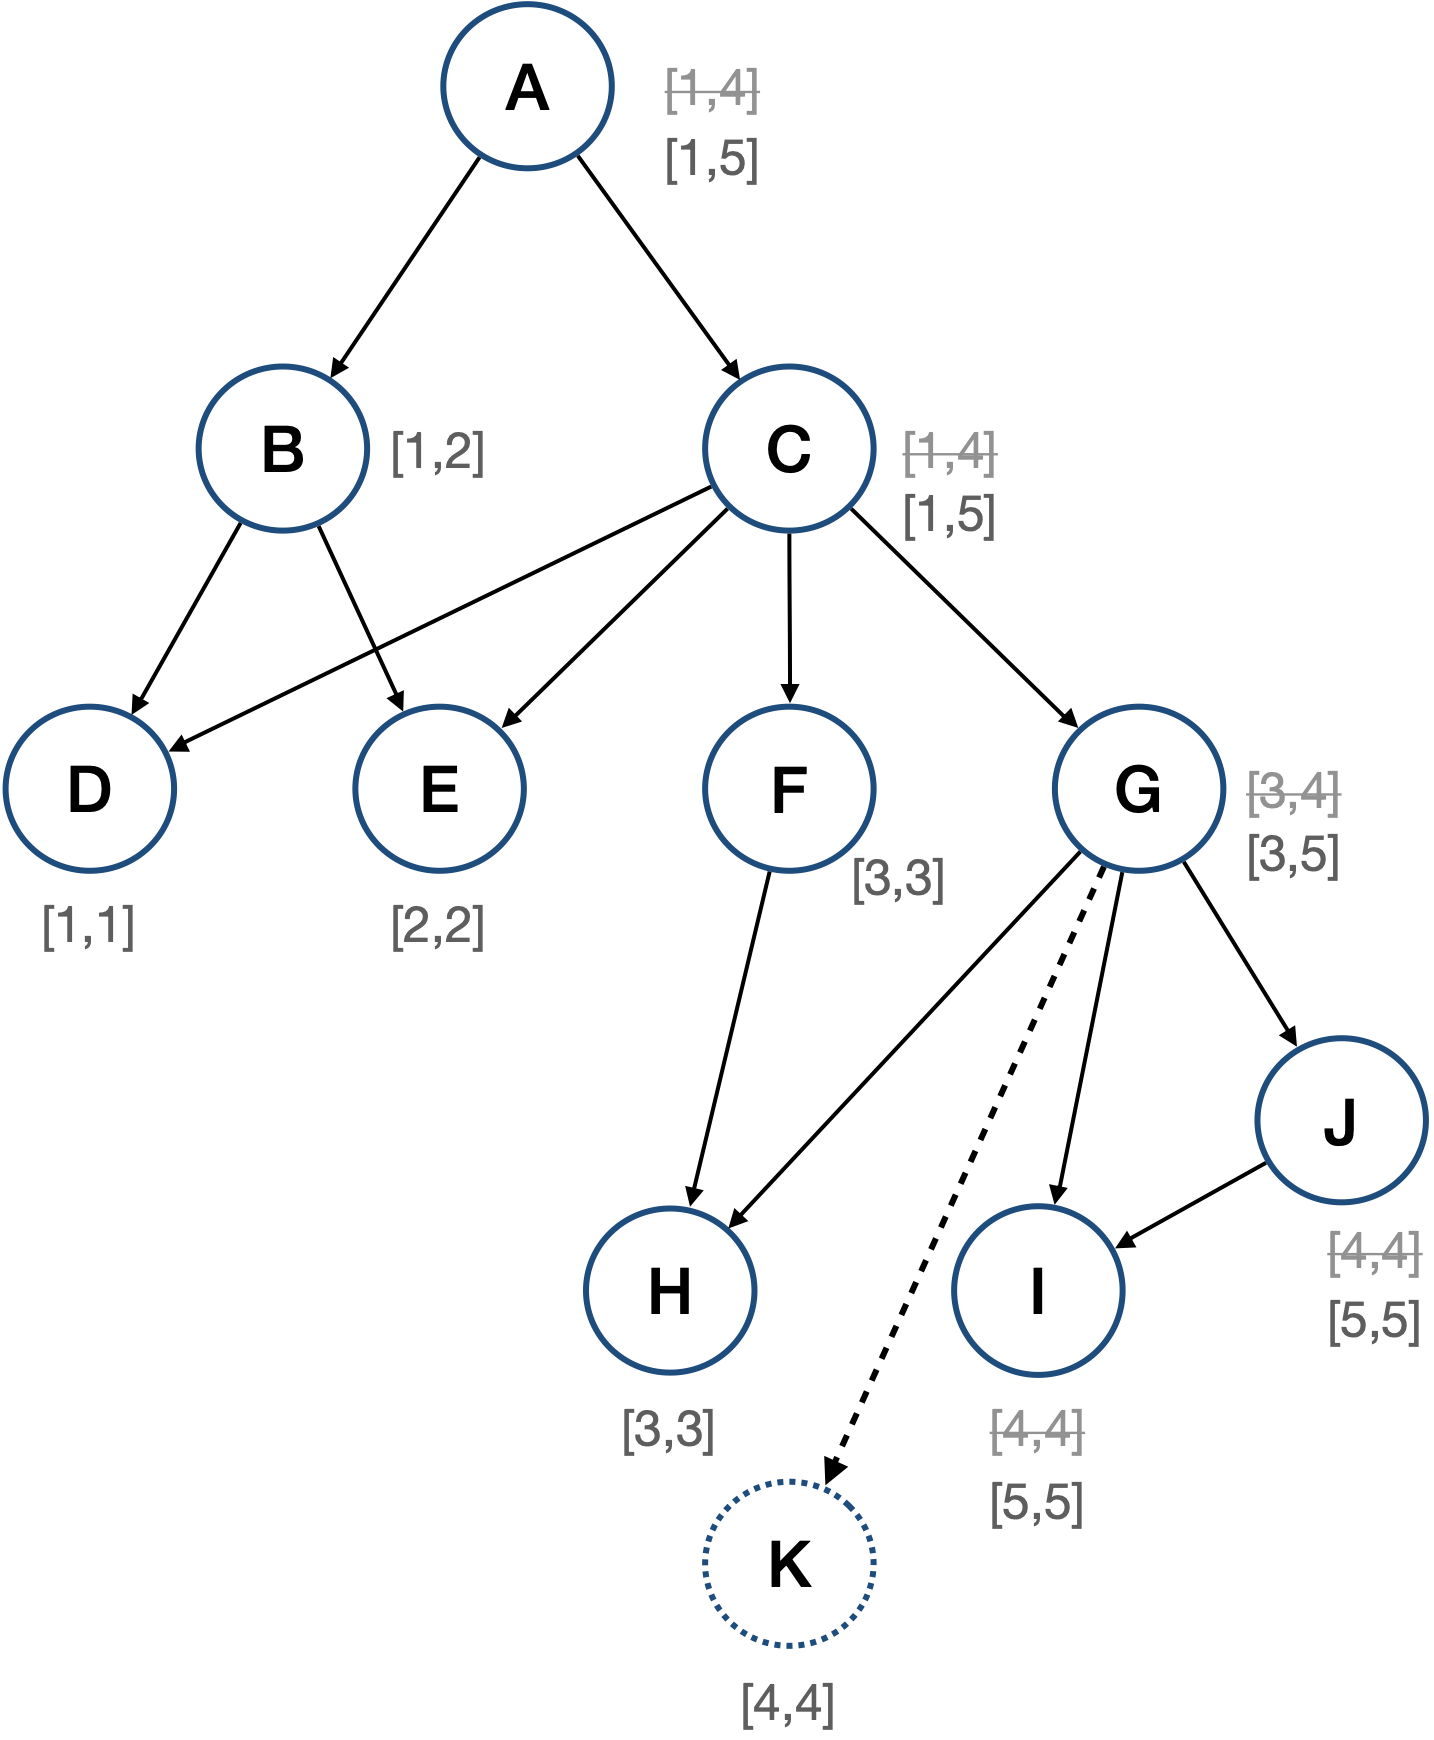
\includegraphics[width=0.6\textwidth]{figures/domlock_example_with_SM.png}
    \caption{DomLock interval recomputation for a vertex insertion}
    \label{fig:domlock_example_SM}
\end{figure}

For example, consider the hierarchy in Figure \ref{fig:domlock_example_SM}. If a vertex $K$ is added as a child of $G$ after $H$, $K$ gets the interval $[4,4]$. $I$ and $J$ get the interval $[5,5]$. Following this, the interval of $G$ is recomputed as $[3,5]$. This recomputation has to be done for all the ancestors of $G$ as well, which includes the root of the hierarchy. 

An additional drawback is that this recomputation is not parallelizable. Since the interval of the root is recomputed as well, any other operation, read, write or structural modification, has to wait until the recomputation is complete. 
This is done in order to prevent incorrect dominator identification due to improper intervals.
In order to prevent concurrent reads from interfering with the recomputation, a mutex has to be placed on the root of the hierarchy. This lock is held until the recomputation is complete. 
In dynamic hierarchies, structural modifications can lead to a significant performance penalty due to the lack of parallelism in the relabelling. 

While DomLock addresses requirements $R1$ and $R2$, false subsumptions and the lack of support for dynamic hierarchies incur significant penalties against requirement $R3$ and $R4$ respectively.



\subsection{Multi Interval DomLock (MID)}
Multi Interval DomLock \cite{anjuMID} is a successor to DomLock which uses a pair of intervals on each vertex to identify the immediate dominator. MID maintains in addition to the DomLock intervals, another interval computed by a reverse post-order traversal of the hierarchy called the \emph{'DFS-on-image'}. Figure \ref{fig:MID_example_locked} shows the MID intervals for a hierarchy. 

\paragraph{Labeling through a pair of numeric intervals}

Each vertex is labelled with two intervals: the \emph{D} interval ($ID_v = [lD_v, rD_v]$) and the \emph{M} interval ($IM = [lM_v, rM_v]$). The only difference between the two intervals is the order of traversal of vertices. D intervals being post-order and M intervals being reverse post-order. Like DomLock, the leaves of the hierarchy are labelled with unit D and M intervals. 
% \begin{figure}[h]
%     \centering
%     \captionsetup{justification=centering}
%     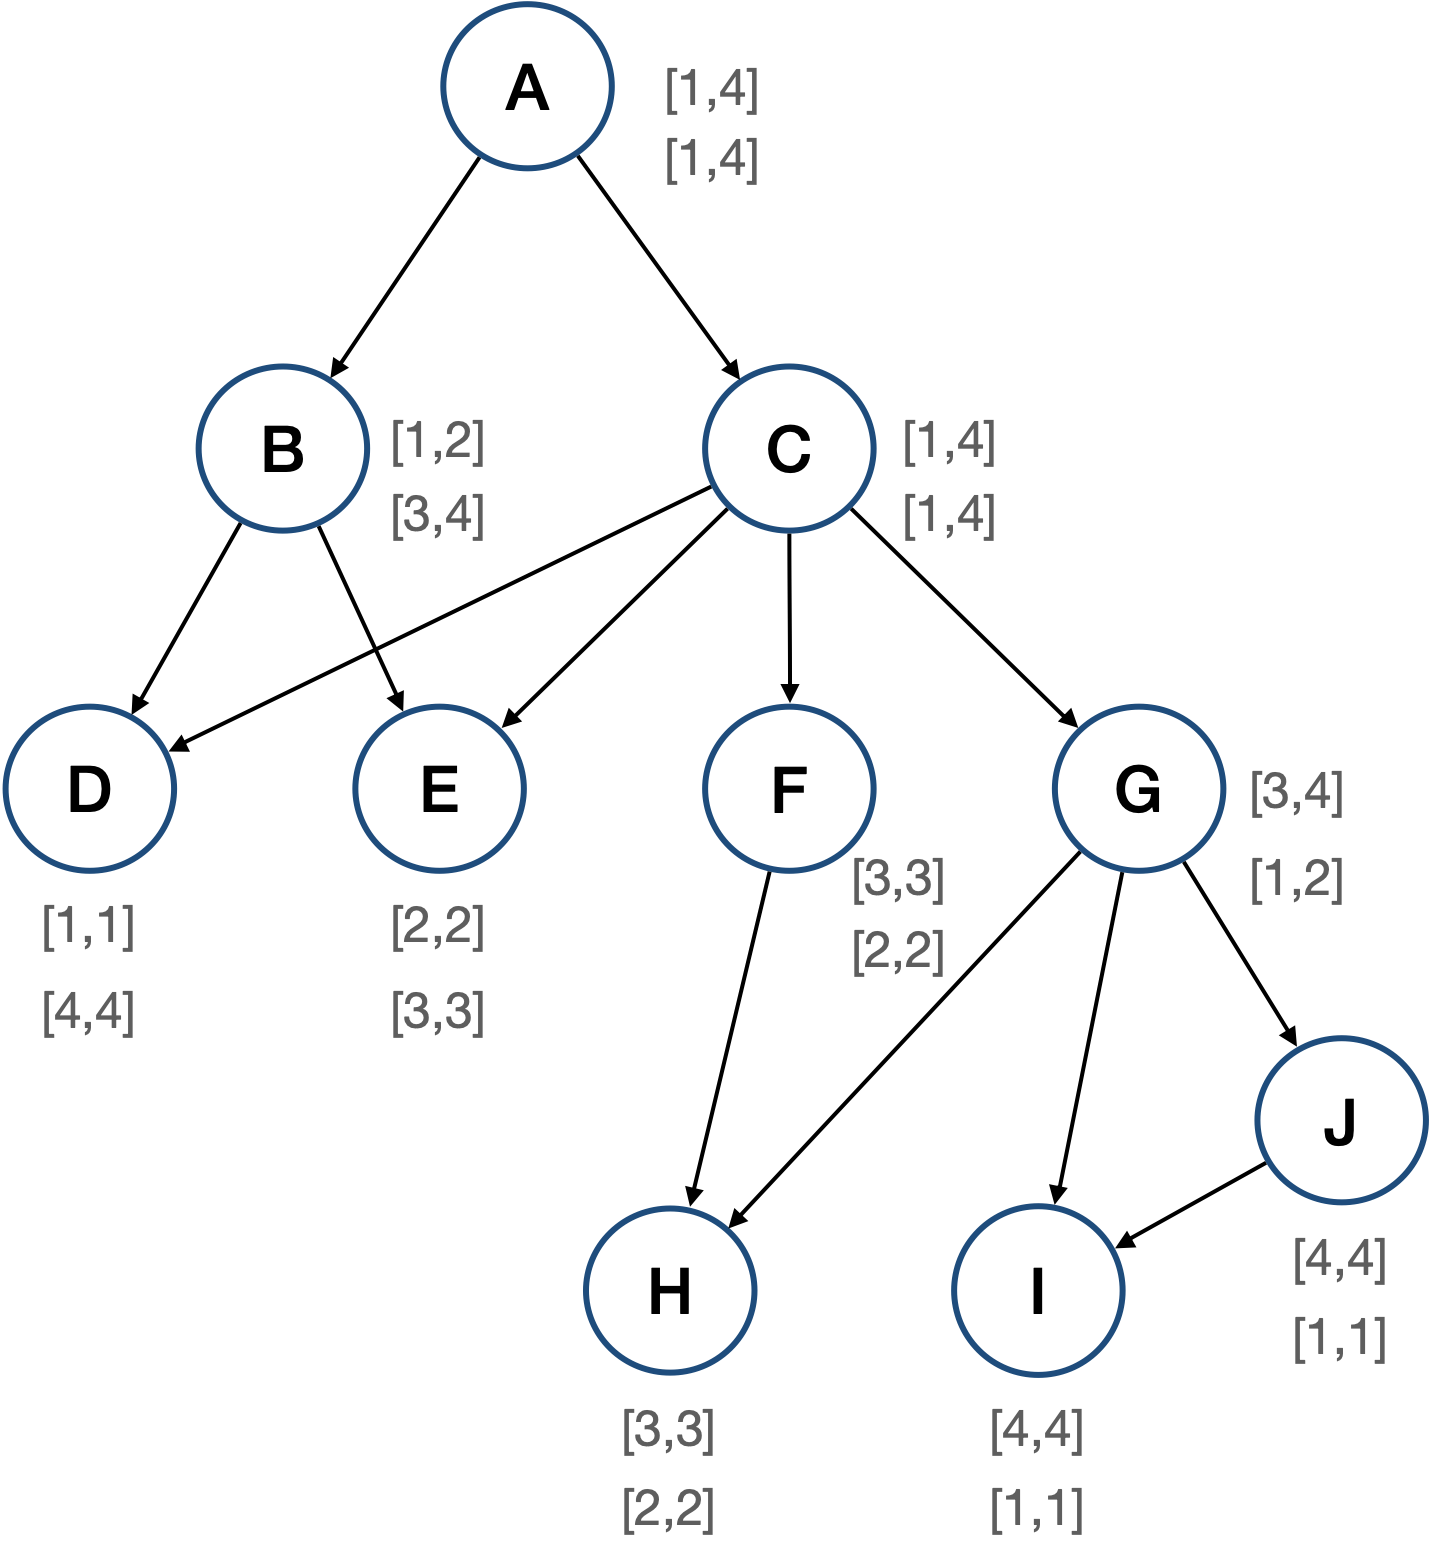
\includegraphics[width=0.5\textwidth]{figures/MID_example.png}
%     \caption{Hierarchy labelled with a pair of intervals: DomLock (top) and MID (bottom)}
%     \label{fig:MID_example}
% \end{figure}

For example, in Figure \ref{fig:MID_example_locked}, vertex $H$ is labelled with a M interval $[2,2]$ in addition to the D interval $[3,3]$ since it is the second vertex in the reverse post-order traversal. Again, like DomLock, for an internal vertex, the interval is computed via the intervals of its children. For both, D and M intervals of a vertex, the $l$ value of an internal vertex $v$ is the minimum of the $l$ values of the D intervals its children and the $r$ value of an internal vertex $v$ is the maximum of the $r$ values of the D intervals of its children.

For example, in Figure \ref{fig:MID_example_locked}, vertex $G$ has three children $H$, $I$ and $J$. The D and M intervals of $G$ are $[3,4]$ and $[1,2]$ respectively since the minimum $l$ value of its children is 3 and 1 and the maximum $r$ value of its children is 4 and 2 respectively.




Intervals of a vertex $v$ subsume ($\prec$) the overlapping intervals of all descendants of $v$. Subsumption is defined as follows:

\begin{equation}
    \begin{split}
        & u \text{ is a dominator of } v \iff ID_u \prec ID_v \land IM_u \prec IM_v
        \\ & \iff lD_v \leq lD_u \land rD_v \geq rD_u \land lM_v \leq lM_u \land rM_v \geq rM_u
    \end{split}
\end{equation}

For example, in Figure \ref{fig:MID_example_locked}, $G$ is a dominator of $F$, $H$, $I$ and $J$ since both D and M intervals of $G$ overlap with the respective D and M intervals of $F$, $H$, $I$ and $J$.

\paragraph{Lock Grain identification}

The property of subsumption is used to identify the lock grain of a guard in MID. However, unlike DomLock, subsumption is tested on both pairs of intervals. While testing subsumption, both D and M intervals are tested for overlap. The grains of two lock guards are disjoint only if both D and M intervals are disjoint. This is done in an effort to reduce the number of false subsumptions. However, as we shall see, MID still suffers from false subsumptions.

% \begin{equation}
    
% \end{equation}


% The two pairs of intervals are used in an attempt to reduce \emph{false subsumptions} where a vertex subsumes its siblings. When testing subsumption in MID, the two intervals are tested for overlap. A vertex $v$ with intervals $[lD_{v1}, r_{v1}]$ and $[l_{v2}, r_{v2}]$, subsumes another vertex $u$ with intervals $[l_{u1}, r_{u1} ]$ and $[l_{u2}, r_{u2}]$ iff $r_{u1} \land l_{u1} \leq r_{v1} \land l_{v2} \leq r_{u2} \land l_{u2} \leq r_{v2}$.

\begin{figure}[H]
    \centering
    \captionsetup{justification=centering}
    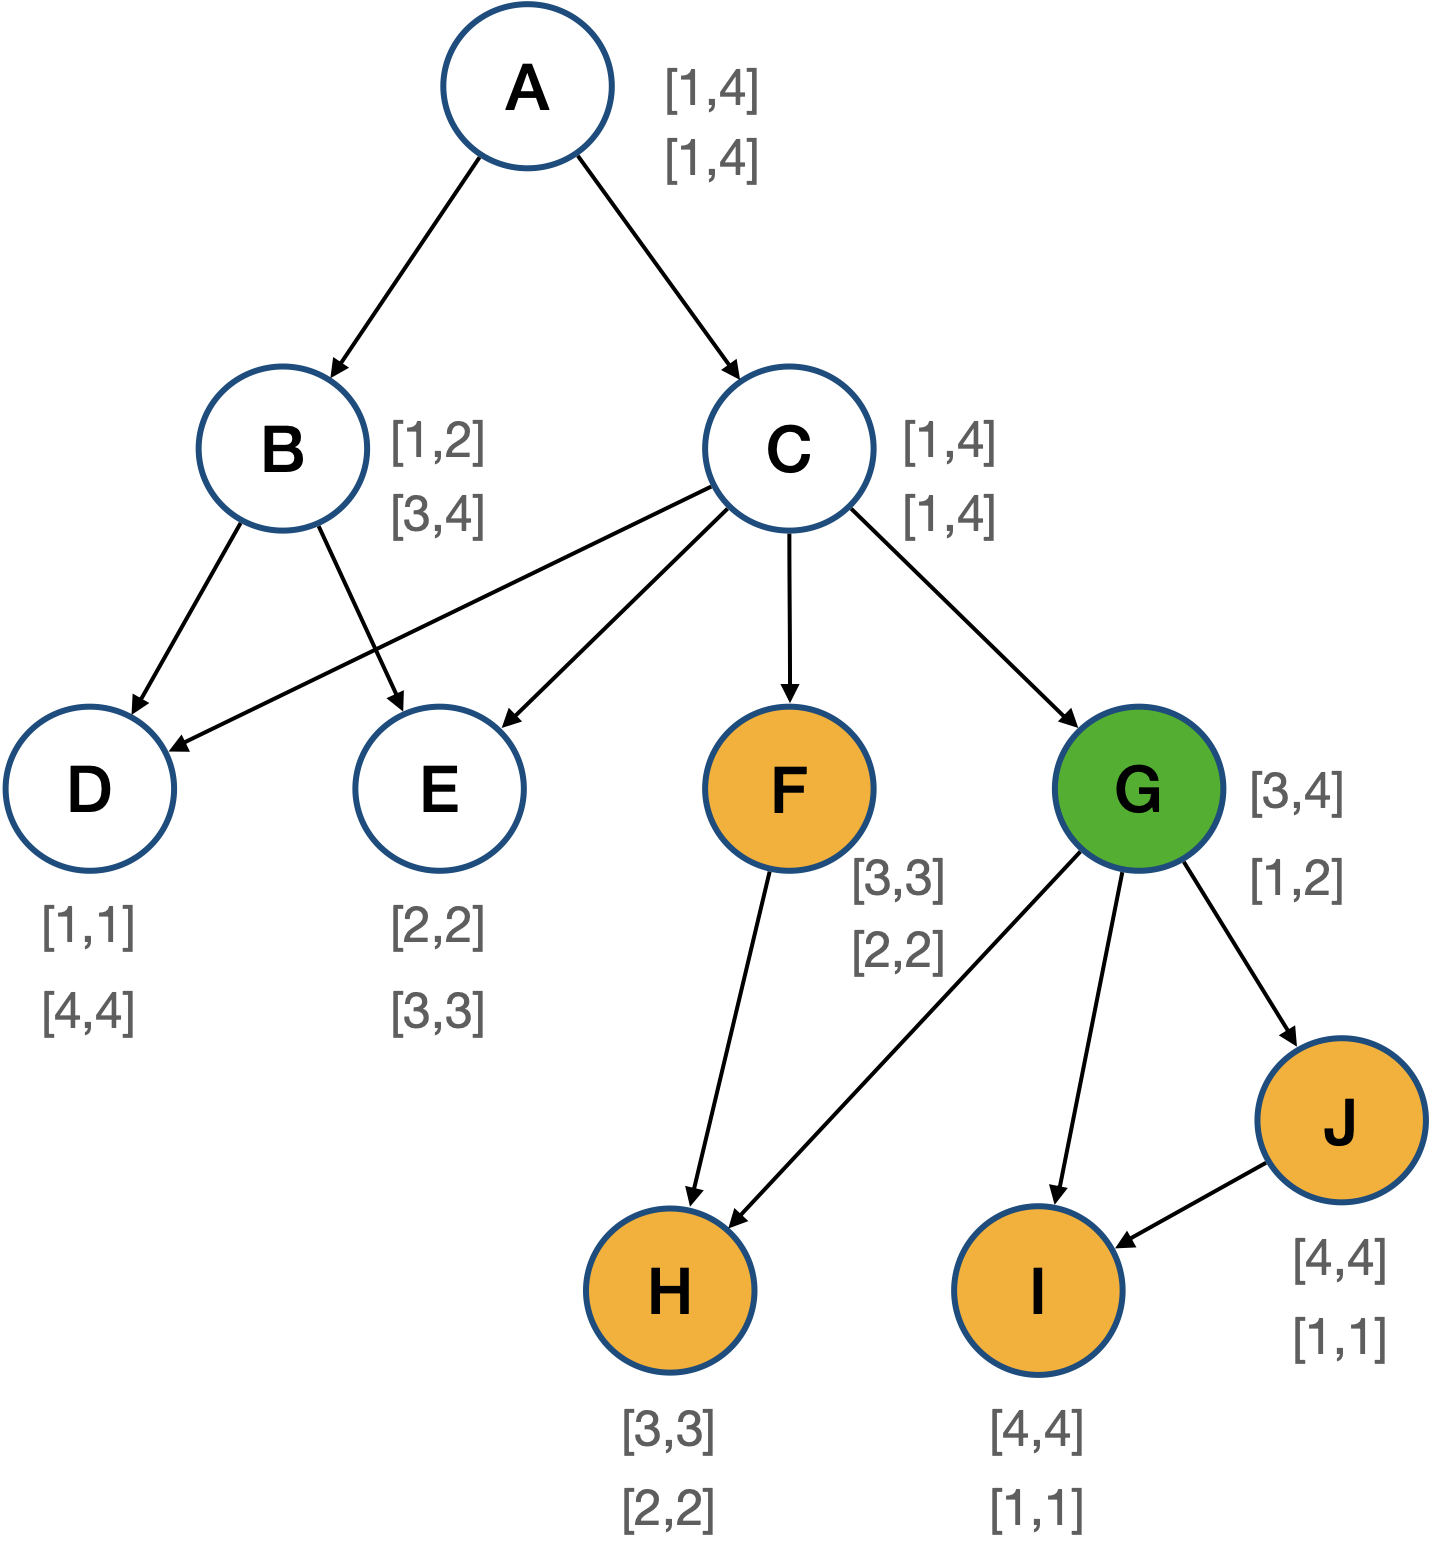
\includegraphics[width=0.6\textwidth]{figures/MID_example_with_lock.png}
    \caption{MID labels with lock on guard $G$ with the grain of the lock (yellow)}
    \label{fig:MID_example_locked}
\end{figure}

For example in Figure \ref{fig:MID_example_locked}, $G$ subsumes $F$, $H$, $I$ and $J$ since both intervals of $G$ overlap with the respective intervals of $F$, $H$, $I$ and $J$. So, Even though MID uses two intervals per vertex, there is still a false subsumption. $G$ subsumes $F$ but $F$ is not a descendant of $G$. A thread that wishes to lock $F$ when $G$ is locked will be blocked due to $F$ and $G$ being included in the same grain even though topologically, they are not. Like DomLock, MID also suffers from poor performance due to such spurious conflicts.

\paragraph{Label recomputation}
MID encounters double the penalty for recomputing vertex labels in dynamic hierarchies when a structural modification occurs. In DomLock, a single post-order traversal is enough to compute all the intervals for a hierarchy. In MID, two traversals are required to compute the intervals when a structural modification occurs. In certain cases, the intervals of all vertices are recomputed which is extremely expensive for large hierarchies.

\begin{figure}[H]
    \centering
    \captionsetup{justification=centering}
    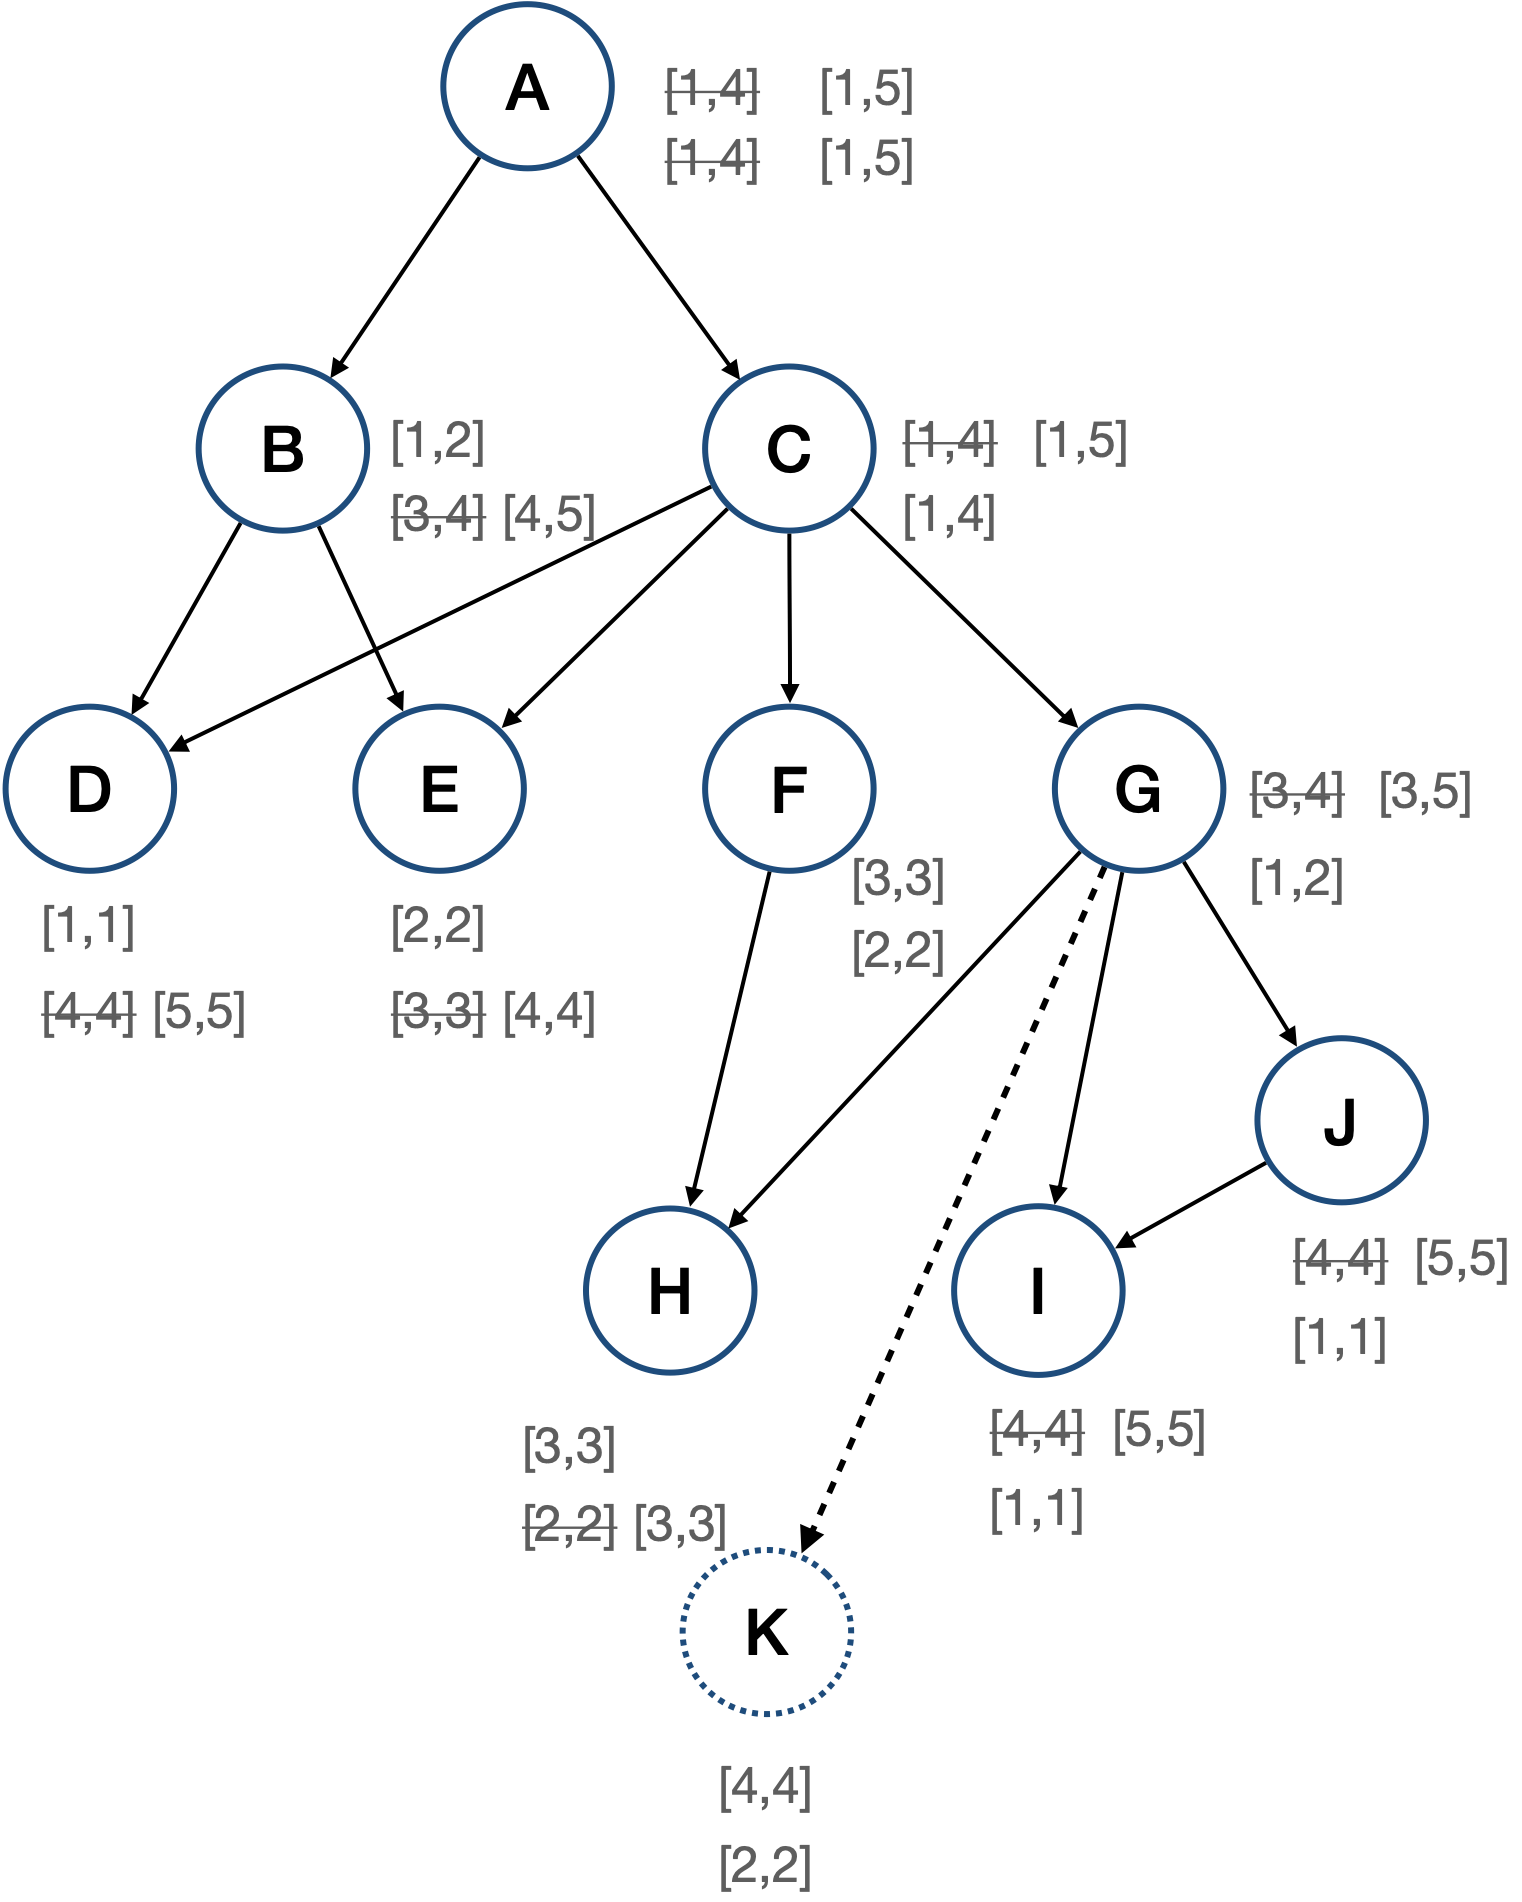
\includegraphics[width=0.6\textwidth]{figures/MID_example_with_SM.png}
    \caption{MID interval recomputation for a vertex insertion}
    \label{fig:MID_example_SM}
    
\end{figure}

For example, when a vertex $K$ is inserted as a child of $G$ as shown in Figure \ref{fig:MID_example_SM}, At least one interval for every vertex is recomputed. These intervals are then propagated to the root of the hierarchy. In order to prevent concurrent reads from interfering with the recomputation, a mutex is acquired on the root of the hierarchy. This lock is held until the recomputation is complete.

MID tries to eliminate false subsumptions present in DomLock but does not do so successfully. The performance penalty for recomputation in dynamic hierarchies is doubled in MID as compared to DomLock. As such, MID fulfills requirements $R1$ and $R2$ but incurs even severe penalties against requirements $R3$ and $R4$ than DomLock.

\subsection{Flexible granularity Locking (FlexiGran)}

FlexiGran \cite{FlexiGran2024} aims to enable the existence of MGL and fixed-grain locks on the same hierarchy. 
DomLock is used as the MGL locking technique in FlexiGran and the fixed-grain locks are fine-grain locks i.e. every vertex is its own guard. 
FlexiGran uses the intervals of DomLock  as vertex labels and uses vertex depth to determine ancestor-descendent relationships between two identical intervals.

\begin{figure}
    \centering
    \captionsetup{justification=centering}
    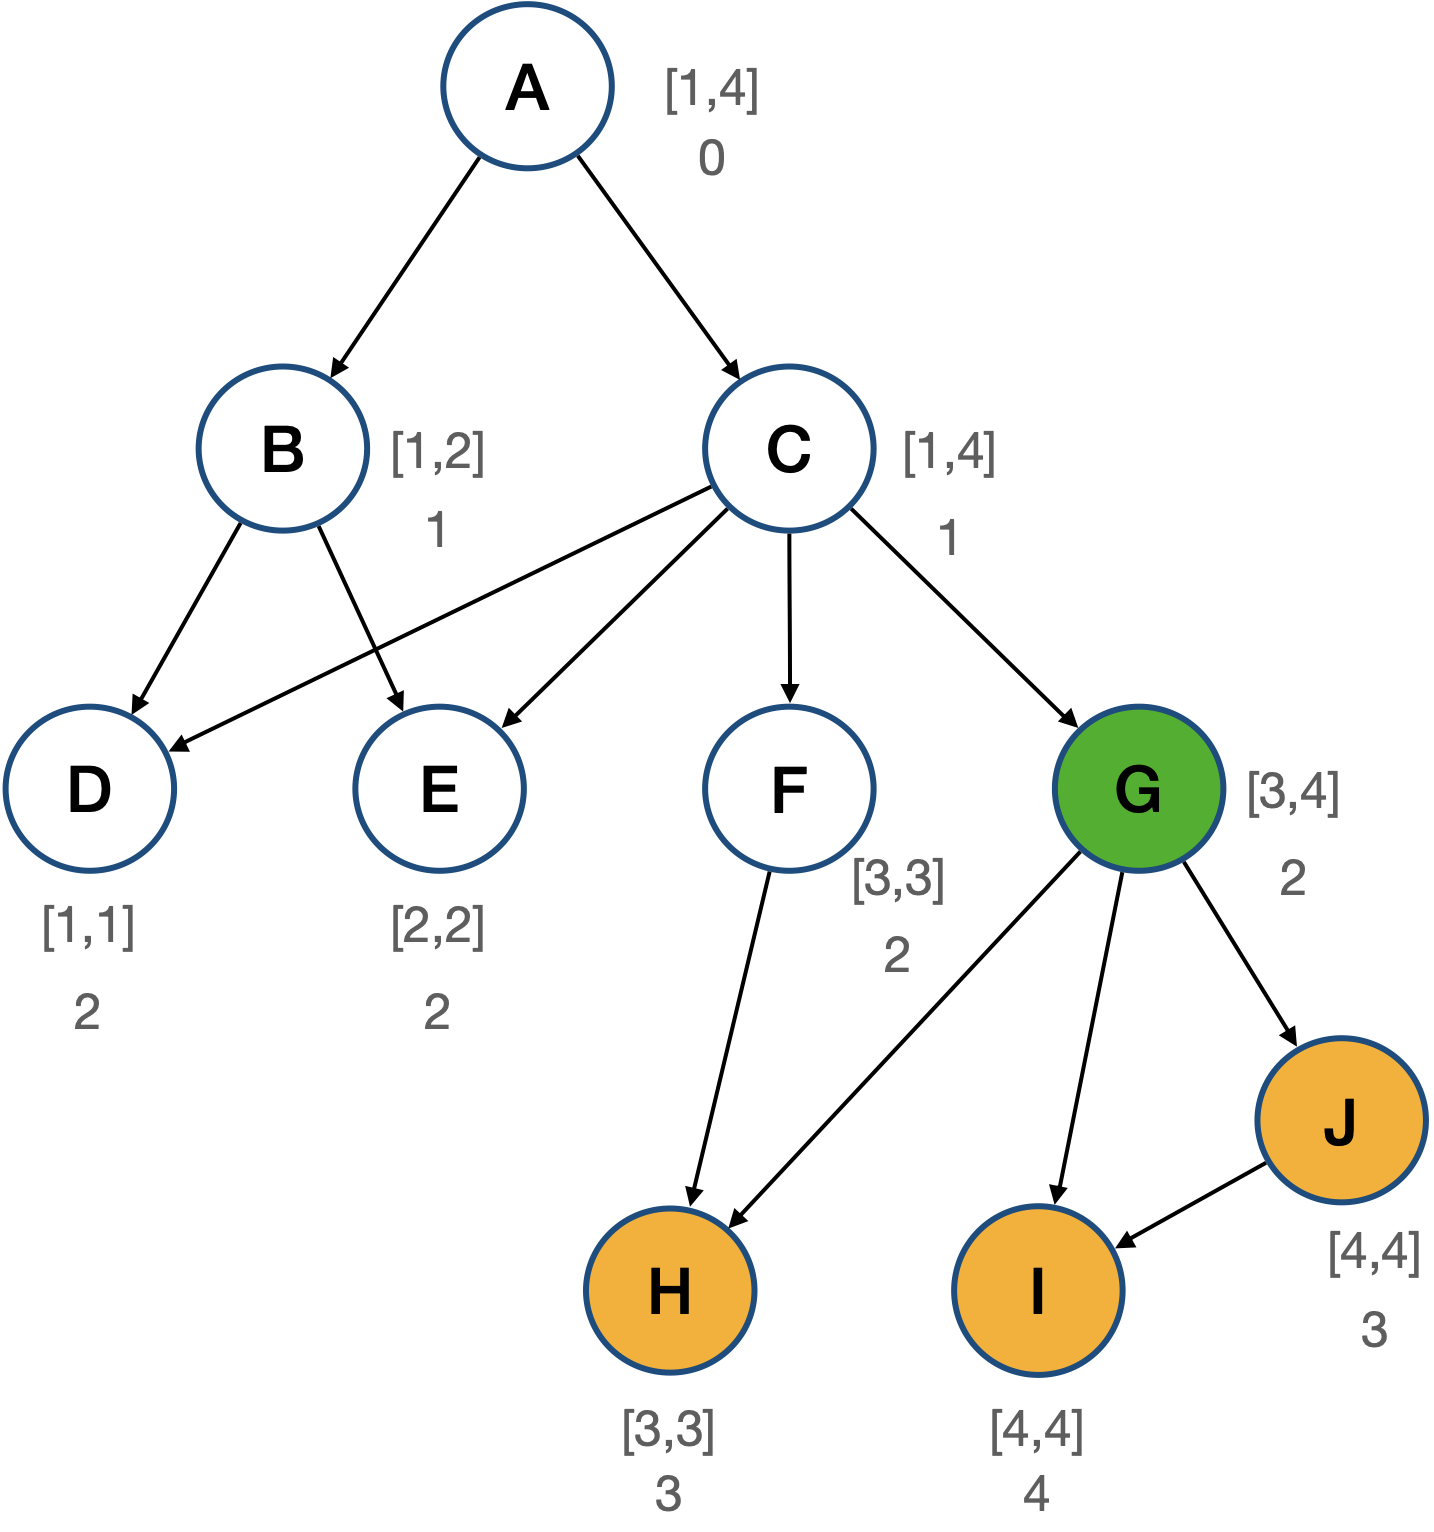
\includegraphics[width=0.5\textwidth]{figures/flexigran_example_with_lock.png}
    \caption{FlexiGran labels and vertex depth with lock on guard $G$ with the grain of the lock (yellow)}
    \label{fig:flexigran_example_locked}
\end{figure}

\paragraph{Labelling through numeric intervals}
In FlexiGran, a post-order traversal is performed to compute the labels of vertices. Like DomLock, the leaves of the hierarchy are labelled with unit intervals and internal vertices are labelled with intervals computed from the intervals of their children. In addition to these intervals, FlexiGran also computes the depth of each vertex in the hierarchy. The depth of a vertex is the length of the shortest-longest path from the root to the vertex. Figure \ref{fig:flexigran_example_locked} shows the intervals and vertex depths of a hierarchy labelled with FlexiGran.

This shortest-longest path is useful for depth determination in the presence of connected components like cycles. In a cycle, the path is recursive and based on the method of computation, the longest path can be infinite. The shortest-longest path breaks this recursion to a limit. This limit is the length of a path from the root to a vertex which contains the target vertex at most twice, as is the case with cycles. 

\paragraph{Lock Grain identification}
FlexiGran uses the depth information in addition to the intervals to determine the ancestor-descendant relationship between two vertices. 
If a thread requests a MGL lock on a vertex via flexigran, then a lock is acquired via the DomLock protocol by performing a depth first search to find the immediate dominator of the target vertex.
If a thread requests a fine-grain lock, then a reader/writer lock is directly requested on the target. 

Since both fine-grain and MGL locks can exist in flexigran, the process of testing lock conflicts involves multiple steps. 

Table \ref{tab:flexigran_locks} shows the compatibility matrix for FlexiGran locks. When checking if two MGL are compatible, the intervals of their guards are tested for overlap. Disjoint intervals indicate that the two locks are DomLock compatible.

When checking two fine-grain locks for conflict, the lock guards for the lock requests are compared. If two fine-grain lock requests are on the same vertex, then they are in conflict if at-least one of the lock requests is for a write lock.


\begin{table}[h]
    \centering
    \captionsetup{justification=centering}
    \begin{tabular}{c|cccc|cccc|}
        \multicolumn{1}{c}{} & \multicolumn{4}{c|}{\textbf{Lock On Ancestor}} & \multicolumn{4}{c}{\textbf{Lock On Descendent}} \\
        \cline{2-9}
        \textbf{Lock Mode} & \textbf{FR} & \textbf{FW} & \textbf{HR} & \textbf{HW} & \textbf{FR} & \textbf{FW} & \textbf{HR} & \textbf{HW} \\
        \hline
        \textbf{FR} & \cellcolor{green!25} Y & \cellcolor{green!25} Y & \cellcolor{green!25} Y & \cellcolor{red!25} N & \cellcolor{green!25} Y & \cellcolor{green!25} Y & \cellcolor{green!25} Y & \cellcolor{green!25} Y \\
        \textbf{FW} & \cellcolor{green!25} Y & \cellcolor{green!25} Y & \cellcolor{red!25} N & \cellcolor{red!25} N & \cellcolor{green!25} Y & \cellcolor{green!25} Y & \cellcolor{green!25} Y & \cellcolor{green!25} Y \\
        \textbf{HR} & \cellcolor{green!25} Y & \cellcolor{green!25} Y & \cellcolor{green!25} Y & \cellcolor{red!25} N & \cellcolor{green!25} Y & \cellcolor{red!25} N & \cellcolor{green!25} Y & \cellcolor{red!25} N \\
        \textbf{HW} & \cellcolor{green!25} Y & \cellcolor{green!25} Y & \cellcolor{red!25} N & \cellcolor{red!25} N & \cellcolor{red!25} N & \cellcolor{red!25} N & \cellcolor{red!25} N & \cellcolor{red!25} N \\
    \end{tabular}
    \caption{Flexigran compatibility matrix showing the protocol for the co-existence of hierarchical and fine-grained locks in a system. \textbf{F}: Fine-grained, \textbf{H}: Hierarchical, \textbf{R}:Read, \textbf{W}: Write}
    \label{tab:flexigran_locks}
\end{table}

To test the compatibility of a MGL lock with a fine-grain lock, it is required to perform an ancestor-descendant relationship check between the guards of the MGL lock and the fine-grain lock. To do so, a traversal is performed and if the fine-grain lock guard is reachable from the MGL lock guard, then the two locks are incompatible since they are related by an ancestor-descendant relationship and are in the same MGL grain. 
For example, in Figure \ref{fig:flexigran_example_locked}, a hierarchical lock is acquired on $G$. This lock guards vertices $H$, $I$ and $J$. Unlike DomLock and MID, FlexiGran does not subsume $F$ since $F$ is not a descendant of $G$ since their depths are the same. In this situation, if a fine-grain lock is requested on $F$, it would be compatible with the hierarchical lock on $G$ since there is no path from $G$ to $F$ or vice-versa.

\paragraph{Label recomputation}
Like DomLock, structural modifications in FlexiGran require recomputation of the intervals of the vertices. A single post-order traversal is enough to recompute the intervals and depths of vertices. Since the root might be involved in the structural modification, a lock is placed on the root to prevent concurrent reads from interfering with the recomputation. This restricts concurrency and leads to a degradation in performance. 

As such, FlexiGran fulfills requirements $R1$ and $R2$ and incurs a significant performance penalty against requirement $R3$ due to the expensive compatibility checks required to detect conflicts between MGL and fine-grain locks. FlexiGran also incurs a performance penalty against requirement $R4$ due to the non-parallel recomputation of intervals in dynamic hierarchies.



\section{Trade-offs between state-of-the-art techniques}

Recall the four primary requirements identified for MGL:
\begin{itemize}
    \item[\textbf{R1}] Identifying a lock guard for every vertex of a hierarchy.
    \item[\textbf{R2}] Finding an appropriate, optimal lock guard for a request.
    \item[\textbf{R3}] Detecting conflicts between locks
    \item[\textbf{R4}] Housekeeping the metadata required to implement the locking protocol.
\end{itemize}

\begin{figure}[h]
    \centering
    \captionsetup{justification=centering}
    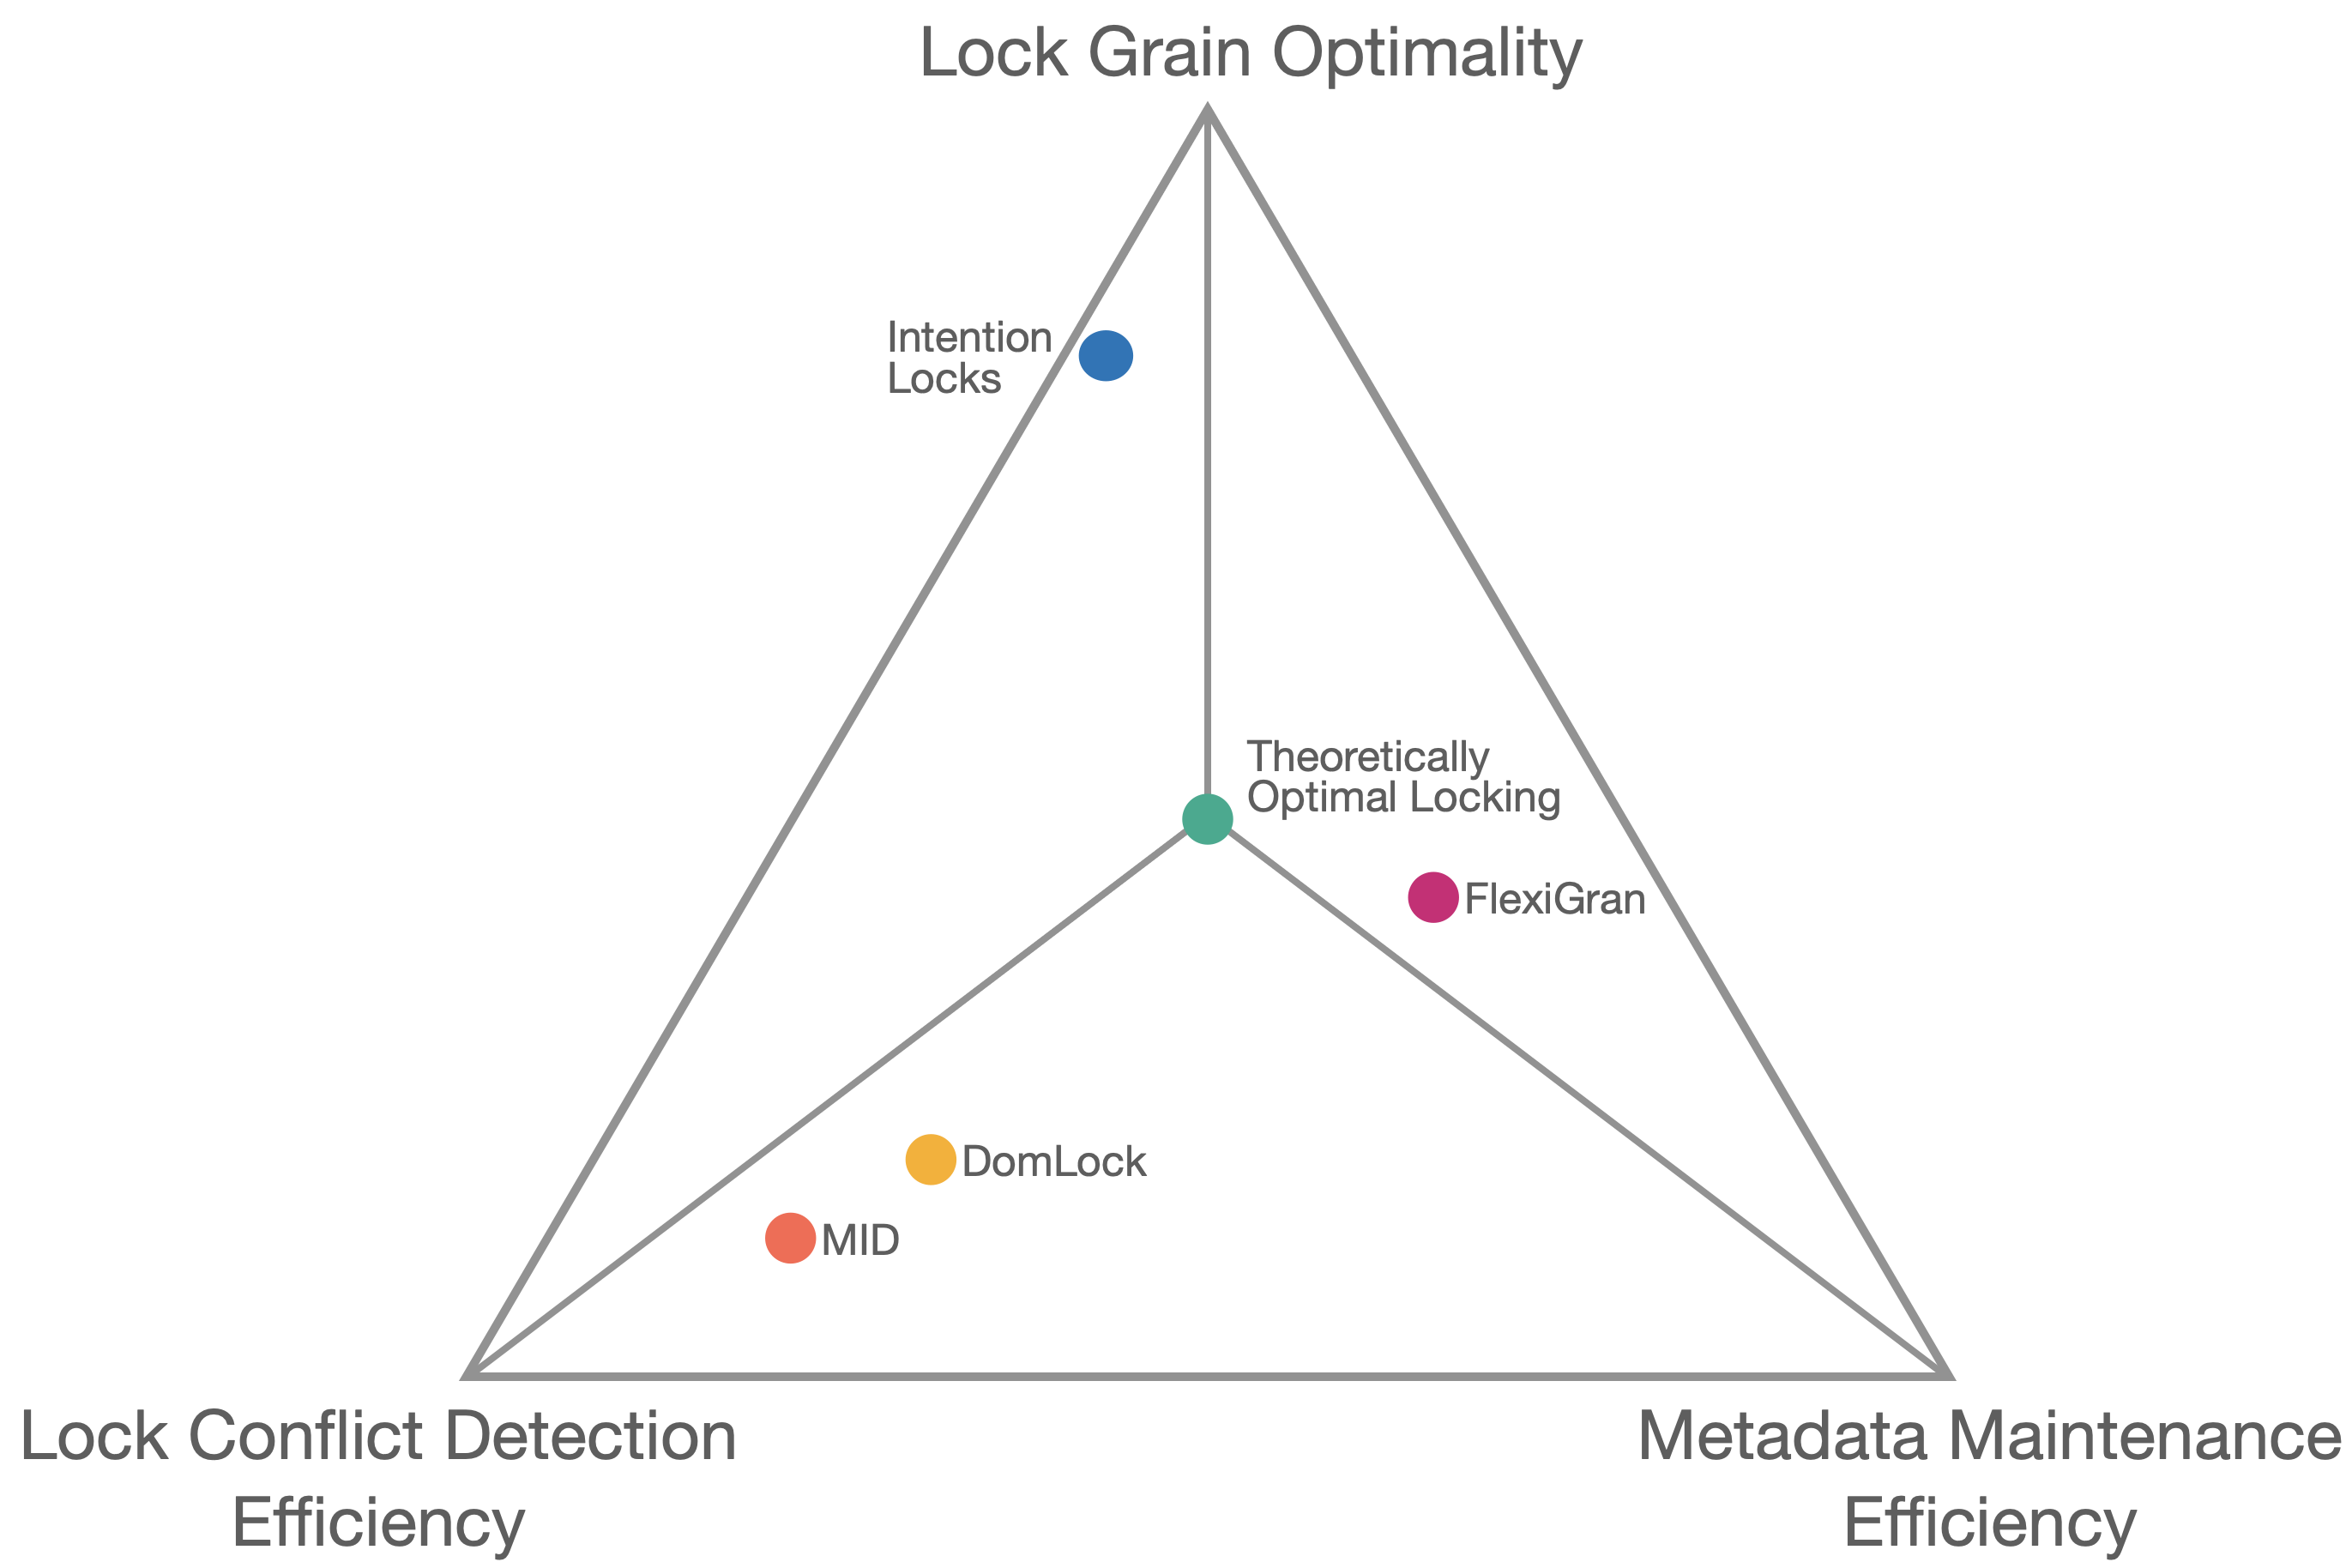
\includegraphics[width=.9\textwidth]{figures/MGL_comparision.png}
    \caption{Trade-offs in MGL techniques}
    \label{fig:tradeoffs}
\end{figure}

Level-based locks are inefficient and only fulfil requirement \textbf{R1}. MGL based on traversals like Intention Lock, fulfills requirements \textbf{R1} and \textbf{R2} but incurs a significant performance penalty against requirement \textbf{R3} due to the sheer number of traversals required to lock a vertex.

Label-based techniques like DomLock, MID and FlexiGran also fulfil requirements \textbf{R1} and \textbf{R2} but incur a performance penalty against requirement \textbf{R3} due to false subsumptions. In addition, due to the metadata required to implement the locking protocol, these techniques incur a performance penalty against requirement \textbf{R4} as well when used in dynamic hierarchies. 
FlexiGran that implements MGL and fine-grain locks suffers from poor performance due to the expensive compatibility checks and label recomputation. 

Figure \ref{fig:tradeoffs} shows the trade-offs in the different MGL techniques. Intention locks offer the most optimal lock grains at the cost of lock conflict detection efficiency. DomLock and MID offer efficient conflict detection at the cost of metadata management. FlexiGran offers better lock grains but incurs a performance penalty due to the expensive lock conflict detection. None of the techniques balances all the requirements to come close to an optimal MGL protocol.


\section{Improving efficiency of MGL techniques}

The locking techniques discussed in chapter \ref{chap:relatedwork} are based on a broad set of assumptions. These assumptions are based either on the topology of the graph or the nature of the workload. Most MGL techniques enforce an ordering of vertices either via reachability thereby utilizing paths to vertices or by a static ordering that ignores the topology of the hierarchy.

\subsection{Path based techniques}
Path based techniques like lock coupling \cite{DBLP:journals/acta/BayerS77}  and intention locks \cite{gray1975granularity} utilize paths from the root of a graph to the lock target. Lock coupling uses a pair of locks that are acquired one after the other on a path to the vertex to prevent concurrent access to the vertex. While intention locking places a set of locks on the path to the vertex to prevent concurrent access. These techniques are efficient for trees and tree-like structures where the path to a vertex from the root is unique. However, generalizing these techniques to graphs or even hierarchies is not appropriate. As we will see in the \ref{chap:evaluation}, the performance of Intention locks degrades significantly when locking over hierarchies.

\subsection{Label based techniques}
Other MGL techniques make use of labelling strategies which identify an ordering of vertices which is later used by the locking protocol to identify the lock guard and grains. Techniques like DomLock, MID and FlexiGran fall into this category. By using a predefined ordering, for example a post-order, these techniques can very efficiently identify the lock guard and grain. However, the topological detail of the graph is lost.  

Other techniques like Toggle \cite{kalikar_toggle_2019} circumvent locking all together and use thread schedulers to prevent race conditions. While scheduling techniques are efficient, they involve redesigning an application and are not readily useable for general developers. 

\subsection{Unified Path and Label based techniques}
Unified techniques for labelling are explored in literature in the domain of metadata management for large scale, efficient searching applications. The Dewey Decimal System \cite{DBLP:journals/jd/Sweeney83} is the earliest example of a path based labelling technique used to identify elements of a hierarchy based on their subclassification. Other path based techniques use similar expensive representations of paths. 

A path based labelling technique that preserves the topological ordering of vertices in the labels and facilitates efficient locking would be an ideal solution. However, the additional metadata required to implement this unified technique should not be prohibitively expensive. DomLock and its successors sacrifice labelling performance for locking performance to an extent that makes them unusable for hierarchies that undergo structural modifications. Our labelling scheme balances maintaining both topological information of the hierarchy while being efficient for locking and also being efficient for relabelling. 

\section{CALock: A topological multi-granularity locking technique}

We propose a new labeling scheme based on path properties, that supports multi-granularity locking. {\em Common-Ancestor lock} ({\em CALock}) is based on a labeling that efficiently computes the closest common ancestor of a set of vertices in a rooted directed graph.
By choosing the closest common ancestor of a set of lock targets as their guard, CALock minimizes grain size. In using paths, by avoiding a fixed ordering of vertices, CALock circumvents expensive relabelling while providing the same locking guarantees as other MGL techniques. The label of a vertex in the graph is a set of its common ancestors, computed recursively via breadth-first traversal which we discuss in chapter \ref{chap:calock}.